\documentclass[twoside]{book}

% Packages required by doxygen
\usepackage{fixltx2e}
\usepackage{calc}
\usepackage{doxygen}
\usepackage[export]{adjustbox} % also loads graphicx
\usepackage{graphicx}
\usepackage[utf8]{inputenc}
\usepackage{makeidx}
\usepackage{multicol}
\usepackage{multirow}
\PassOptionsToPackage{warn}{textcomp}
\usepackage{textcomp}
\usepackage[nointegrals]{wasysym}
\usepackage[table]{xcolor}

% Font selection
\usepackage[T1]{fontenc}
\usepackage[scaled=.90]{helvet}
\usepackage{courier}
\usepackage{amssymb}
\usepackage{sectsty}
\renewcommand{\familydefault}{\sfdefault}
\allsectionsfont{%
  \fontseries{bc}\selectfont%
  \color{darkgray}%
}
\renewcommand{\DoxyLabelFont}{%
  \fontseries{bc}\selectfont%
  \color{darkgray}%
}
\newcommand{\+}{\discretionary{\mbox{\scriptsize$\hookleftarrow$}}{}{}}

% Page & text layout
\usepackage{geometry}
\geometry{%
  a4paper,%
  top=2.5cm,%
  bottom=2.5cm,%
  left=2.5cm,%
  right=2.5cm%
}
\tolerance=750
\hfuzz=15pt
\hbadness=750
\setlength{\emergencystretch}{15pt}
\setlength{\parindent}{0cm}
\setlength{\parskip}{3ex plus 2ex minus 2ex}
\makeatletter
\renewcommand{\paragraph}{%
  \@startsection{paragraph}{4}{0ex}{-1.0ex}{1.0ex}{%
    \normalfont\normalsize\bfseries\SS@parafont%
  }%
}
\renewcommand{\subparagraph}{%
  \@startsection{subparagraph}{5}{0ex}{-1.0ex}{1.0ex}{%
    \normalfont\normalsize\bfseries\SS@subparafont%
  }%
}
\makeatother

% Headers & footers
\usepackage{fancyhdr}
\pagestyle{fancyplain}
\fancyhead[LE]{\fancyplain{}{\bfseries\thepage}}
\fancyhead[CE]{\fancyplain{}{}}
\fancyhead[RE]{\fancyplain{}{\bfseries\leftmark}}
\fancyhead[LO]{\fancyplain{}{\bfseries\rightmark}}
\fancyhead[CO]{\fancyplain{}{}}
\fancyhead[RO]{\fancyplain{}{\bfseries\thepage}}
\fancyfoot[LE]{\fancyplain{}{}}
\fancyfoot[CE]{\fancyplain{}{}}
\fancyfoot[RE]{\fancyplain{}{\bfseries\scriptsize Generated by Doxygen }}
\fancyfoot[LO]{\fancyplain{}{\bfseries\scriptsize Generated by Doxygen }}
\fancyfoot[CO]{\fancyplain{}{}}
\fancyfoot[RO]{\fancyplain{}{}}
\renewcommand{\footrulewidth}{0.4pt}
\renewcommand{\chaptermark}[1]{%
  \markboth{#1}{}%
}
\renewcommand{\sectionmark}[1]{%
  \markright{\thesection\ #1}%
}

% Indices & bibliography
\usepackage{natbib}
\usepackage[titles]{tocloft}
\setcounter{tocdepth}{3}
\setcounter{secnumdepth}{5}
\makeindex

% Custom commands
\newcommand{\clearemptydoublepage}{%
  \newpage{\pagestyle{empty}\cleardoublepage}%
}

\usepackage{caption}
\captionsetup{labelsep=space,justification=centering,font={bf},singlelinecheck=off,skip=4pt,position=top}

%===== C O N T E N T S =====

\begin{document}

% Titlepage & ToC
\pagenumbering{alph}
\begin{titlepage}
\vspace*{7cm}
\begin{center}%
{\Large Ksiegarnia }\\
\vspace*{1cm}
{\large Generated by Doxygen 1.8.13}\\
\end{center}
\end{titlepage}
\clearemptydoublepage
\pagenumbering{roman}
\tableofcontents
\clearemptydoublepage
\pagenumbering{arabic}

%--- Begin generated contents ---
\chapter{Hierarchical Index}
\section{Class Hierarchy}
This inheritance list is sorted roughly, but not completely, alphabetically\+:\begin{DoxyCompactList}
\item \contentsline{section}{Ksiazka}{\pageref{class_ksiazka}}{}
\item \contentsline{section}{Pracownicy}{\pageref{class_pracownicy}}{}
\item \contentsline{section}{Przedsiebiorstwo}{\pageref{class_przedsiebiorstwo}}{}
\begin{DoxyCompactList}
\item \contentsline{section}{Drukarnia}{\pageref{class_drukarnia}}{}
\item \contentsline{section}{Ksiegarnia}{\pageref{class_ksiegarnia}}{}
\begin{DoxyCompactList}
\item \contentsline{section}{Ksiegarnia\+Internetowa}{\pageref{class_ksiegarnia_internetowa}}{}
\end{DoxyCompactList}
\end{DoxyCompactList}
\item \contentsline{section}{Siedziba}{\pageref{class_siedziba}}{}
\end{DoxyCompactList}

\chapter{Class Index}
\section{Class List}
Here are the classes, structs, unions and interfaces with brief descriptions\+:\begin{DoxyCompactList}
\item\contentsline{section}{\textbf{ Drukarnia} \\*Klasa \doxyref{Drukarnia}{p.}{class_drukarnia}, pochodna klasy \doxyref{Przedsiebiorstwo}{p.}{class_przedsiebiorstwo} }{\pageref{class_drukarnia}}{}
\item\contentsline{section}{\textbf{ Ksiazka} \\*Klasa przechowujaca dane o ksiazkach znajdujacych sie w ksiegarni }{\pageref{class_ksiazka}}{}
\item\contentsline{section}{\textbf{ Ksiegarnia} \\*Klasa \doxyref{Ksiegarnia}{p.}{class_ksiegarnia}, pochodna klasy \doxyref{Przedsiebiorstwo}{p.}{class_przedsiebiorstwo} }{\pageref{class_ksiegarnia}}{}
\item\contentsline{section}{\textbf{ Ksiegarnia\+Internetowa} \\*Klasa \doxyref{Ksiegarnia}{p.}{class_ksiegarnia} Internetowa, pochodna klasy \doxyref{Ksiegarnia}{p.}{class_ksiegarnia} }{\pageref{class_ksiegarnia_internetowa}}{}
\item\contentsline{section}{\textbf{ Pracownicy} \\*Klasa przechowujaca dane o pracownikach firmy }{\pageref{class_pracownicy}}{}
\item\contentsline{section}{\textbf{ Przedsiebiorstwo} \\*Klasa abstrakcyjna }{\pageref{class_przedsiebiorstwo}}{}
\item\contentsline{section}{\textbf{ Siedziba} \\*Klasa przechowujaca dane o siedzibie firmy }{\pageref{class_siedziba}}{}
\end{DoxyCompactList}

\chapter{File Index}
\section{File List}
Here is a list of all files with brief descriptions\+:\begin{DoxyCompactList}
\item\contentsline{section}{\textbf{ Drukarnia.\+cpp} }{\pageref{_drukarnia_8cpp}}{}
\item\contentsline{section}{\textbf{ Drukarnia.\+h} }{\pageref{_drukarnia_8h}}{}
\item\contentsline{section}{\textbf{ Ksiazka.\+cpp} }{\pageref{_ksiazka_8cpp}}{}
\item\contentsline{section}{\textbf{ Ksiazka.\+h} }{\pageref{_ksiazka_8h}}{}
\item\contentsline{section}{\textbf{ Ksiegarnia internetowa.\+cpp} }{\pageref{_ksiegarnia_01internetowa_8cpp}}{}
\item\contentsline{section}{\textbf{ Ksiegarnia internetowa.\+h} }{\pageref{_ksiegarnia_01internetowa_8h}}{}
\item\contentsline{section}{\textbf{ Ksiegarnia.\+cpp} }{\pageref{_ksiegarnia_8cpp}}{}
\item\contentsline{section}{\textbf{ Ksiegarnia.\+h} }{\pageref{_ksiegarnia_8h}}{}
\item\contentsline{section}{\textbf{ Pracownicy.\+cpp} }{\pageref{_pracownicy_8cpp}}{}
\item\contentsline{section}{\textbf{ Pracownicy.\+h} }{\pageref{_pracownicy_8h}}{}
\item\contentsline{section}{\textbf{ Program.\+cpp} }{\pageref{_program_8cpp}}{}
\item\contentsline{section}{\textbf{ Przedsiebiorstwo.\+cpp} }{\pageref{_przedsiebiorstwo_8cpp}}{}
\item\contentsline{section}{\textbf{ Przedsiebiorstwo.\+h} }{\pageref{_przedsiebiorstwo_8h}}{}
\item\contentsline{section}{\textbf{ Siedziba.\+cpp} }{\pageref{_siedziba_8cpp}}{}
\item\contentsline{section}{\textbf{ Siedziba.\+h} }{\pageref{_siedziba_8h}}{}
\item\contentsline{section}{\textbf{ stdafx.\+cpp} }{\pageref{stdafx_8cpp}}{}
\item\contentsline{section}{\textbf{ stdafx.\+h} }{\pageref{stdafx_8h}}{}
\item\contentsline{section}{\textbf{ targetver.\+h} }{\pageref{targetver_8h}}{}
\end{DoxyCompactList}

\chapter{Class Documentation}
\section{Drukarnia Class Reference}
\label{class_drukarnia}\index{Drukarnia@{Drukarnia}}


Klasa \doxyref{Drukarnia}{p.}{class_drukarnia}, pochodna klasy \doxyref{Przedsiebiorstwo}{p.}{class_przedsiebiorstwo}.  




{\ttfamily \#include $<$Drukarnia.\+h$>$}

Inheritance diagram for Drukarnia\+:\begin{figure}[H]
\begin{center}
\leavevmode
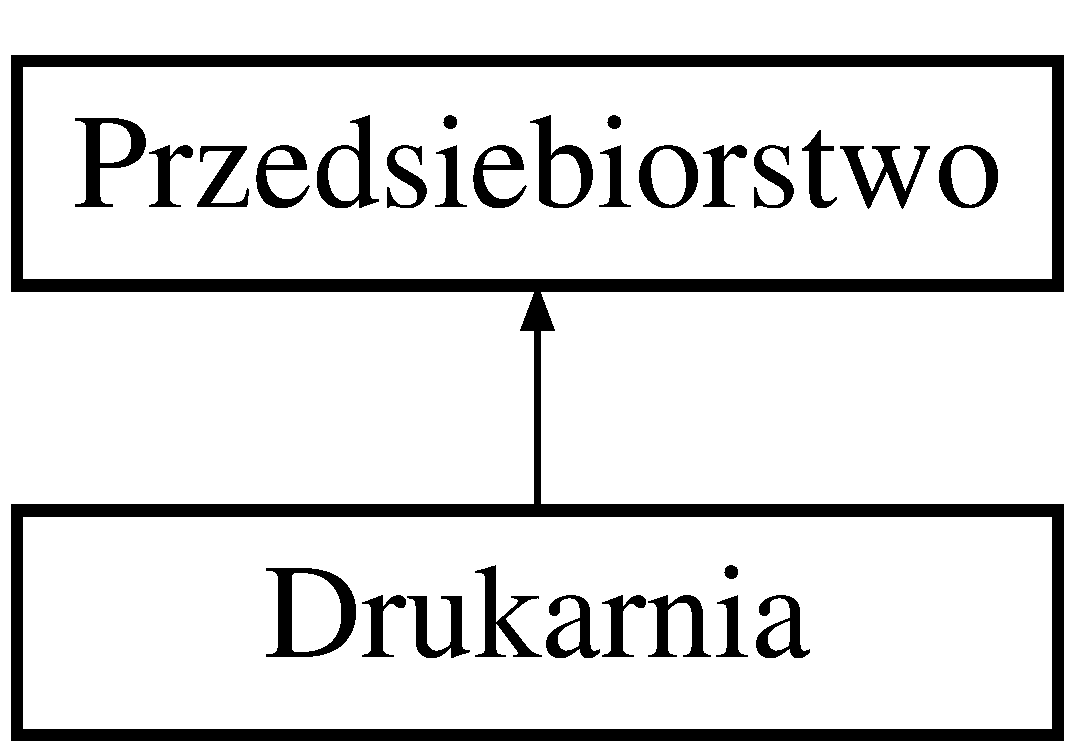
\includegraphics[height=2.000000cm]{class_drukarnia}
\end{center}
\end{figure}
\subsection*{Public Member Functions}
\begin{DoxyCompactItemize}
\item 
\textbf{ Drukarnia} ()
\begin{DoxyCompactList}\small\item\em Kontruktor domyslny. \end{DoxyCompactList}\item 
\textbf{ $\sim$\+Drukarnia} ()
\begin{DoxyCompactList}\small\item\em Destruktor. \end{DoxyCompactList}\item 
void \textbf{ wypisz\+Dane\+Firmy} (ostream \&s)
\begin{DoxyCompactList}\small\item\em Metoda pozwalajaca uzyskac dane na temat Drukarni. \end{DoxyCompactList}\item 
void \textbf{ wprowadz\+Dane\+Firmy\+Z\+Pliku} (istream \&s)
\begin{DoxyCompactList}\small\item\em Metoda pozwalajaca na wprowadzenie danych Drukarni. \end{DoxyCompactList}\item 
void \textbf{ wprowadz\+Dane\+Drukarni} (string nowa\+\_\+nazwa, string nowy\+\_\+adres, int nowa\+\_\+ilosc\+\_\+drukarek, int nowy\+\_\+telefon)
\begin{DoxyCompactList}\small\item\em Metoda pozwalajaca wprowadzic dane drukarni. \end{DoxyCompactList}\end{DoxyCompactItemize}
\subsection*{Static Public Attributes}
\begin{DoxyCompactItemize}
\item 
static int \textbf{ ilosc\+Drukarni} = 0
\end{DoxyCompactItemize}
\subsection*{Protected Attributes}
\begin{DoxyCompactItemize}
\item 
string \textbf{ nazwa}
\begin{DoxyCompactList}\small\item\em Zmienna przechowujaca nazwe drukarni. \end{DoxyCompactList}\item 
int \textbf{ ilosc\+\_\+drukarek}
\begin{DoxyCompactList}\small\item\em Zmienna przechowujaca liczbe drukarek znajdujacych sie w drukarni. \end{DoxyCompactList}\end{DoxyCompactItemize}
\subsection*{Friends}
\begin{DoxyCompactItemize}
\item 
ostream \& \textbf{ operator$<$$<$} (ostream \&s, \textbf{ Drukarnia} \&d)
\begin{DoxyCompactList}\small\item\em Zaprzyjazniony operator strumieniowy. \end{DoxyCompactList}\item 
istream \& \textbf{ operator$>$$>$} (istream \&s, \textbf{ Drukarnia} \&d)
\begin{DoxyCompactList}\small\item\em Zaprzyjazniony operator strumieniowy. \end{DoxyCompactList}\end{DoxyCompactItemize}
\subsection*{Additional Inherited Members}


\subsection{Detailed Description}
Klasa \doxyref{Drukarnia}{p.}{class_drukarnia}, pochodna klasy \doxyref{Przedsiebiorstwo}{p.}{class_przedsiebiorstwo}. 

\subsection{Constructor \& Destructor Documentation}
\mbox{\label{class_drukarnia_af421887bf3ea71bfa41a6cbeecbb84fa}} 
\index{Drukarnia@{Drukarnia}!Drukarnia@{Drukarnia}}
\index{Drukarnia@{Drukarnia}!Drukarnia@{Drukarnia}}
\subsubsection{Drukarnia()}
{\footnotesize\ttfamily Drukarnia\+::\+Drukarnia (\begin{DoxyParamCaption}{ }\end{DoxyParamCaption})}



Kontruktor domyslny. 

\mbox{\label{class_drukarnia_a6873a3fc7c08bb7bb6dbceb9c9e4bfda}} 
\index{Drukarnia@{Drukarnia}!````~Drukarnia@{$\sim$\+Drukarnia}}
\index{````~Drukarnia@{$\sim$\+Drukarnia}!Drukarnia@{Drukarnia}}
\subsubsection{$\sim$\+Drukarnia()}
{\footnotesize\ttfamily Drukarnia\+::$\sim$\+Drukarnia (\begin{DoxyParamCaption}{ }\end{DoxyParamCaption})}



Destruktor. 



\subsection{Member Function Documentation}
\mbox{\label{class_drukarnia_a5c5e6859eacaa7603857dc2597d43781}} 
\index{Drukarnia@{Drukarnia}!wprowadz\+Dane\+Drukarni@{wprowadz\+Dane\+Drukarni}}
\index{wprowadz\+Dane\+Drukarni@{wprowadz\+Dane\+Drukarni}!Drukarnia@{Drukarnia}}
\subsubsection{wprowadz\+Dane\+Drukarni()}
{\footnotesize\ttfamily void Drukarnia\+::wprowadz\+Dane\+Drukarni (\begin{DoxyParamCaption}\item[{string}]{nowa\+\_\+nazwa,  }\item[{string}]{nowy\+\_\+adres,  }\item[{int}]{nowa\+\_\+ilosc\+\_\+drukarek,  }\item[{int}]{nowy\+\_\+telefon }\end{DoxyParamCaption})}



Metoda pozwalajaca wprowadzic dane drukarni. 

Metoda pozwala na dodanie nazwy, adresu, ilosci drukarek i nr telefonu drukarni. 
\begin{DoxyParams}{Parameters}
{\em nowa\+\_\+nazwa} & nazwa drukarni \\
\hline
{\em nowy\+\_\+adres} & adres drukarni \\
\hline
{\em nowa\+\_\+ilosc\+\_\+drukarek} & ilosc drukarek w drukarni \\
\hline
{\em nowy\+\_\+telefon} & telefon do drukarni \\
\hline
\end{DoxyParams}
\mbox{\label{class_drukarnia_aa77de3fe83557754ebac4a6b4a443c9d}} 
\index{Drukarnia@{Drukarnia}!wprowadz\+Dane\+Firmy\+Z\+Pliku@{wprowadz\+Dane\+Firmy\+Z\+Pliku}}
\index{wprowadz\+Dane\+Firmy\+Z\+Pliku@{wprowadz\+Dane\+Firmy\+Z\+Pliku}!Drukarnia@{Drukarnia}}
\subsubsection{wprowadz\+Dane\+Firmy\+Z\+Pliku()}
{\footnotesize\ttfamily void Drukarnia\+::wprowadz\+Dane\+Firmy\+Z\+Pliku (\begin{DoxyParamCaption}\item[{istream \&}]{s }\end{DoxyParamCaption})\hspace{0.3cm}{\ttfamily [virtual]}}



Metoda pozwalajaca na wprowadzenie danych Drukarni. 

Umozliwia wprowadzanie danych obiektu z pliku. 
\begin{DoxyParams}{Parameters}
{\em s} & strumien wejscia \\
\hline
\end{DoxyParams}


Reimplemented from \textbf{ Przedsiebiorstwo} \doxyref{}{p.}{class_przedsiebiorstwo_adff311023ef04e492b6a7db7d4a8a01c}.

\mbox{\label{class_drukarnia_a9ebed3c69bdb7fbc30dfca3fda086233}} 
\index{Drukarnia@{Drukarnia}!wypisz\+Dane\+Firmy@{wypisz\+Dane\+Firmy}}
\index{wypisz\+Dane\+Firmy@{wypisz\+Dane\+Firmy}!Drukarnia@{Drukarnia}}
\subsubsection{wypisz\+Dane\+Firmy()}
{\footnotesize\ttfamily void Drukarnia\+::wypisz\+Dane\+Firmy (\begin{DoxyParamCaption}\item[{ostream \&}]{s }\end{DoxyParamCaption})\hspace{0.3cm}{\ttfamily [virtual]}}



Metoda pozwalajaca uzyskac dane na temat Drukarni. 

Umozliwia wyprowadzenie danych obiektu na dowolny strumien wyjscia. 
\begin{DoxyParams}{Parameters}
{\em s} & dowolny strumien wyjscia \\
\hline
\end{DoxyParams}


Implements \textbf{ Przedsiebiorstwo} \doxyref{}{p.}{class_przedsiebiorstwo_aff6ca5801f0160b5201be2209c58459d}.



\subsection{Friends And Related Function Documentation}
\mbox{\label{class_drukarnia_a0980f69a891e6b38b5bba72efa182ef9}} 
\index{Drukarnia@{Drukarnia}!operator$<$$<$@{operator$<$$<$}}
\index{operator$<$$<$@{operator$<$$<$}!Drukarnia@{Drukarnia}}
\subsubsection{operator$<$$<$}
{\footnotesize\ttfamily ostream\& operator$<$$<$ (\begin{DoxyParamCaption}\item[{ostream \&}]{s,  }\item[{\textbf{ Drukarnia} \&}]{d }\end{DoxyParamCaption})\hspace{0.3cm}{\ttfamily [friend]}}



Zaprzyjazniony operator strumieniowy. 

Przeciazony operator pozwala na uzyskanie danych na dowlny strumien wyjscia. W tym programie wykorzystywany do wypisu danych na standardowe wyjscie lub do pliku. \mbox{\label{class_drukarnia_af4a4c25098d3c4c31f1f16d79bedeaa9}} 
\index{Drukarnia@{Drukarnia}!operator$>$$>$@{operator$>$$>$}}
\index{operator$>$$>$@{operator$>$$>$}!Drukarnia@{Drukarnia}}
\subsubsection{operator$>$$>$}
{\footnotesize\ttfamily istream\& operator$>$$>$ (\begin{DoxyParamCaption}\item[{istream \&}]{s,  }\item[{\textbf{ Drukarnia} \&}]{d }\end{DoxyParamCaption})\hspace{0.3cm}{\ttfamily [friend]}}



Zaprzyjazniony operator strumieniowy. 

Przeciazony operator pozwala na pobranie danych z dowolnego strumienia wejscia. W tym programie wykorzystywany do odczytu danych z pliku. 

\subsection{Member Data Documentation}
\mbox{\label{class_drukarnia_a8ad27d8287cfa41d2b6b1269bf88d711}} 
\index{Drukarnia@{Drukarnia}!ilosc\+\_\+drukarek@{ilosc\+\_\+drukarek}}
\index{ilosc\+\_\+drukarek@{ilosc\+\_\+drukarek}!Drukarnia@{Drukarnia}}
\subsubsection{ilosc\+\_\+drukarek}
{\footnotesize\ttfamily int Drukarnia\+::ilosc\+\_\+drukarek\hspace{0.3cm}{\ttfamily [protected]}}



Zmienna przechowujaca liczbe drukarek znajdujacych sie w drukarni. 

\mbox{\label{class_drukarnia_a624b645d2d5b74df14404081b3bf70e6}} 
\index{Drukarnia@{Drukarnia}!ilosc\+Drukarni@{ilosc\+Drukarni}}
\index{ilosc\+Drukarni@{ilosc\+Drukarni}!Drukarnia@{Drukarnia}}
\subsubsection{ilosc\+Drukarni}
{\footnotesize\ttfamily int Drukarnia\+::ilosc\+Drukarni = 0\hspace{0.3cm}{\ttfamily [static]}}

zmienna przechowujaca ilosc utworzonych obiektow (Drukarni) \mbox{\label{class_drukarnia_ae0546df33f7cf9055b3418fef4854919}} 
\index{Drukarnia@{Drukarnia}!nazwa@{nazwa}}
\index{nazwa@{nazwa}!Drukarnia@{Drukarnia}}
\subsubsection{nazwa}
{\footnotesize\ttfamily string Drukarnia\+::nazwa\hspace{0.3cm}{\ttfamily [protected]}}



Zmienna przechowujaca nazwe drukarni. 



The documentation for this class was generated from the following files\+:\begin{DoxyCompactItemize}
\item 
\textbf{ Drukarnia.\+h}\item 
\textbf{ Drukarnia.\+cpp}\end{DoxyCompactItemize}

\section{Ksiazka Class Reference}
\label{class_ksiazka}\index{Ksiazka@{Ksiazka}}


Klasa przechowujaca dane o ksiazkach znajdujacych sie w ksiegarni.  




{\ttfamily \#include $<$Ksiazka.\+h$>$}

\subsection*{Public Member Functions}
\begin{DoxyCompactItemize}
\item 
\textbf{ Ksiazka} ()
\begin{DoxyCompactList}\small\item\em Konstruktor domyslny. \end{DoxyCompactList}\item 
\textbf{ Ksiazka} (string nowy\+\_\+tytul, string nowy\+\_\+autor, int nowy\+\_\+rok\+\_\+wydania)
\begin{DoxyCompactList}\small\item\em Konstruktor z parametrami. \end{DoxyCompactList}\item 
\textbf{ $\sim$\+Ksiazka} ()
\begin{DoxyCompactList}\small\item\em Destruktor. \end{DoxyCompactList}\end{DoxyCompactItemize}
\subsection*{Friends}
\begin{DoxyCompactItemize}
\item 
ostream \& \textbf{ operator$<$$<$} (ostream \&s, \textbf{ Ksiazka} \&k)
\begin{DoxyCompactList}\small\item\em Zaprzyjazniony operator strumieniowy. \end{DoxyCompactList}\end{DoxyCompactItemize}


\subsection{Detailed Description}
Klasa przechowujaca dane o ksiazkach znajdujacych sie w ksiegarni. 

\subsection{Constructor \& Destructor Documentation}
\mbox{\label{class_ksiazka_a97f373a60dd715626284eb900bcfbd6b}} 
\index{Ksiazka@{Ksiazka}!Ksiazka@{Ksiazka}}
\index{Ksiazka@{Ksiazka}!Ksiazka@{Ksiazka}}
\subsubsection{Ksiazka()\hspace{0.1cm}{\footnotesize\ttfamily [1/2]}}
{\footnotesize\ttfamily Ksiazka\+::\+Ksiazka (\begin{DoxyParamCaption}{ }\end{DoxyParamCaption})}



Konstruktor domyslny. 

\mbox{\label{class_ksiazka_aeff8f7a776d569b3eff2181b1afb0949}} 
\index{Ksiazka@{Ksiazka}!Ksiazka@{Ksiazka}}
\index{Ksiazka@{Ksiazka}!Ksiazka@{Ksiazka}}
\subsubsection{Ksiazka()\hspace{0.1cm}{\footnotesize\ttfamily [2/2]}}
{\footnotesize\ttfamily Ksiazka\+::\+Ksiazka (\begin{DoxyParamCaption}\item[{string}]{nowy\+\_\+tytul,  }\item[{string}]{nowy\+\_\+autor,  }\item[{int}]{nowy\+\_\+rok\+\_\+wydania }\end{DoxyParamCaption})}



Konstruktor z parametrami. 

\mbox{\label{class_ksiazka_accf293b1b1b7a8ac5ffe28decfd6400c}} 
\index{Ksiazka@{Ksiazka}!````~Ksiazka@{$\sim$\+Ksiazka}}
\index{````~Ksiazka@{$\sim$\+Ksiazka}!Ksiazka@{Ksiazka}}
\subsubsection{$\sim$\+Ksiazka()}
{\footnotesize\ttfamily Ksiazka\+::$\sim$\+Ksiazka (\begin{DoxyParamCaption}{ }\end{DoxyParamCaption})}



Destruktor. 



\subsection{Friends And Related Function Documentation}
\mbox{\label{class_ksiazka_a6304f50ce62c067a686efe441f71c54d}} 
\index{Ksiazka@{Ksiazka}!operator$<$$<$@{operator$<$$<$}}
\index{operator$<$$<$@{operator$<$$<$}!Ksiazka@{Ksiazka}}
\subsubsection{operator$<$$<$}
{\footnotesize\ttfamily ostream\& operator$<$$<$ (\begin{DoxyParamCaption}\item[{ostream \&}]{s,  }\item[{\textbf{ Ksiazka} \&}]{k }\end{DoxyParamCaption})\hspace{0.3cm}{\ttfamily [friend]}}



Zaprzyjazniony operator strumieniowy. 

Przeciazony operator pozwala na uzyskanie danych na dowolny strumien wyjscia. W tym programie wykorzystywany do wypisu danych na standardowe wyjscie lub do pliku. 

The documentation for this class was generated from the following files\+:\begin{DoxyCompactItemize}
\item 
\textbf{ Ksiazka.\+h}\item 
\textbf{ Ksiazka.\+cpp}\end{DoxyCompactItemize}

\section{Ksiegarnia Class Reference}
\label{class_ksiegarnia}\index{Ksiegarnia@{Ksiegarnia}}


Klasa \doxyref{Ksiegarnia}{p.}{class_ksiegarnia}, pochodna klasy \doxyref{Przedsiebiorstwo}{p.}{class_przedsiebiorstwo}.  




{\ttfamily \#include $<$Ksiegarnia.\+h$>$}

Inheritance diagram for Ksiegarnia\+:\begin{figure}[H]
\begin{center}
\leavevmode
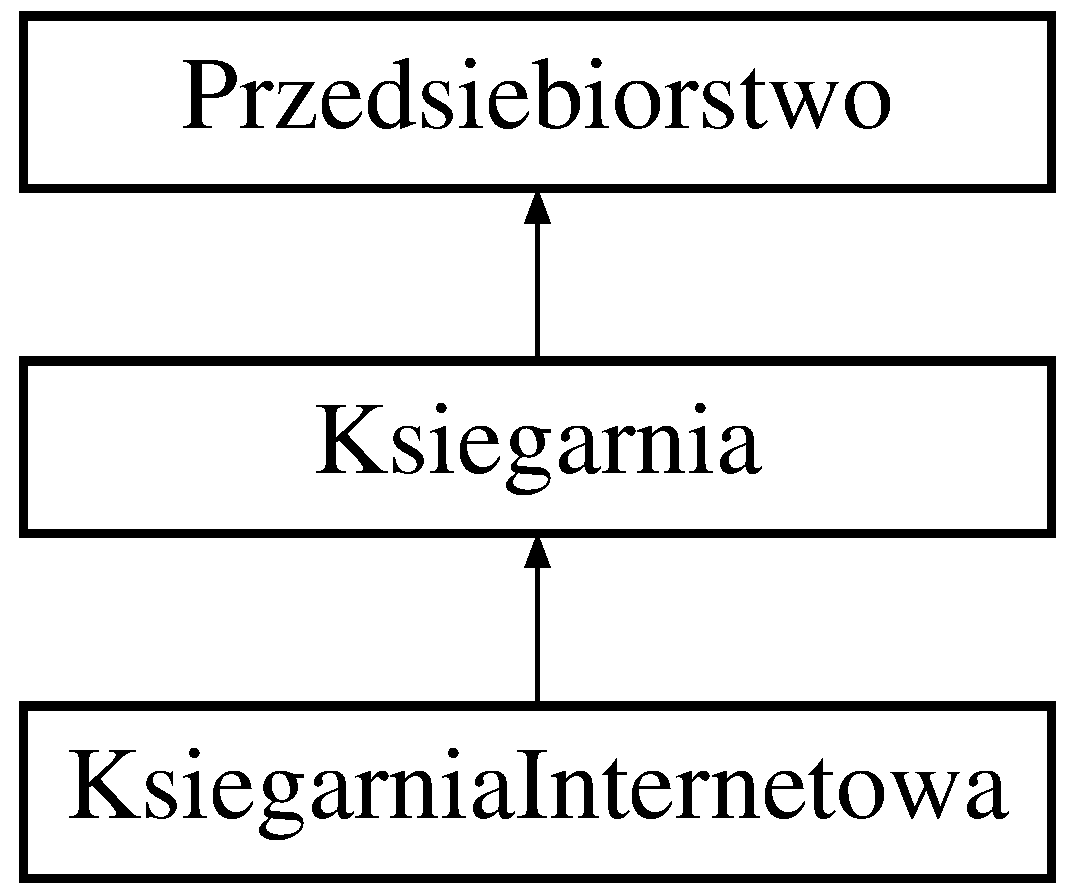
\includegraphics[height=3.000000cm]{class_ksiegarnia}
\end{center}
\end{figure}
\subsection*{Public Member Functions}
\begin{DoxyCompactItemize}
\item 
\textbf{ Ksiegarnia} ()
\begin{DoxyCompactList}\small\item\em domyslny konstruktor \end{DoxyCompactList}\item 
\textbf{ $\sim$\+Ksiegarnia} ()
\begin{DoxyCompactList}\small\item\em destruktor \end{DoxyCompactList}\item 
void \textbf{ dodaj\+Ksiazke} (string tytul, string autor, int rok\+\_\+wydania)
\begin{DoxyCompactList}\small\item\em Metoda pozwalajaca dodac ksiazke do Ksiegarni. \end{DoxyCompactList}\item 
void \textbf{ usun\+Ksiazke} (int ktora)
\begin{DoxyCompactList}\small\item\em Metoda pozwalajaca usunac ksiazke z Ksiegarni. \end{DoxyCompactList}\item 
void \textbf{ wypisz\+Dane\+Firmy} (ostream \&s)
\begin{DoxyCompactList}\small\item\em Metoda pozwalajaca uzyskac dane na temat Ksiegarni. \end{DoxyCompactList}\item 
void \textbf{ wprowadz\+Dane\+Firmy\+Z\+Pliku} (istream \&s)
\begin{DoxyCompactList}\small\item\em Metoda pozwalajaca na wprowadzenie danych Ksiegarni. \end{DoxyCompactList}\item 
void \textbf{ wprowadz\+Dane\+Ksiegarni} (string nowa\+\_\+nazwa, string nowy\+\_\+adres, int nowy\+\_\+telefon)
\begin{DoxyCompactList}\small\item\em Metoda pozwalajaca wprowadzic dane Ksiegarni. \end{DoxyCompactList}\end{DoxyCompactItemize}
\subsection*{Static Public Attributes}
\begin{DoxyCompactItemize}
\item 
static int \textbf{ ilosc\+Ksiegarni} = 0
\end{DoxyCompactItemize}
\subsection*{Protected Attributes}
\begin{DoxyCompactItemize}
\item 
string \textbf{ nazwa}
\begin{DoxyCompactList}\small\item\em zmienna przechowujaca nazwe ksiegarni \end{DoxyCompactList}\item 
vector$<$ \textbf{ Ksiazka} $>$ \textbf{ ksiazka}
\begin{DoxyCompactList}\small\item\em kontener zawierajacy dane ksiazek znajdujacych sie w Ksiegarni \end{DoxyCompactList}\end{DoxyCompactItemize}
\subsection*{Friends}
\begin{DoxyCompactItemize}
\item 
istream \& \textbf{ operator$>$$>$} (istream \&s, \textbf{ Ksiegarnia} \&k)
\begin{DoxyCompactList}\small\item\em Zaprzyjazniony operator strumieniowy. \end{DoxyCompactList}\item 
ostream \& \textbf{ operator$<$$<$} (ostream \&s, \textbf{ Ksiegarnia} \&k)
\begin{DoxyCompactList}\small\item\em Zaprzyjazniony operator strumieniowy. \end{DoxyCompactList}\end{DoxyCompactItemize}
\subsection*{Additional Inherited Members}


\subsection{Detailed Description}
Klasa \doxyref{Ksiegarnia}{p.}{class_ksiegarnia}, pochodna klasy \doxyref{Przedsiebiorstwo}{p.}{class_przedsiebiorstwo}. 

\subsection{Constructor \& Destructor Documentation}
\mbox{\label{class_ksiegarnia_a1aa6512e422dfeb7b849c9a037c55348}} 
\index{Ksiegarnia@{Ksiegarnia}!Ksiegarnia@{Ksiegarnia}}
\index{Ksiegarnia@{Ksiegarnia}!Ksiegarnia@{Ksiegarnia}}
\subsubsection{Ksiegarnia()}
{\footnotesize\ttfamily Ksiegarnia\+::\+Ksiegarnia (\begin{DoxyParamCaption}{ }\end{DoxyParamCaption})}



domyslny konstruktor 

\mbox{\label{class_ksiegarnia_a01d78ac29e0f15c72eeb213005b52d07}} 
\index{Ksiegarnia@{Ksiegarnia}!````~Ksiegarnia@{$\sim$\+Ksiegarnia}}
\index{````~Ksiegarnia@{$\sim$\+Ksiegarnia}!Ksiegarnia@{Ksiegarnia}}
\subsubsection{$\sim$\+Ksiegarnia()}
{\footnotesize\ttfamily Ksiegarnia\+::$\sim$\+Ksiegarnia (\begin{DoxyParamCaption}{ }\end{DoxyParamCaption})}



destruktor 



\subsection{Member Function Documentation}
\mbox{\label{class_ksiegarnia_ae16987b405a6f3f8a7d4e44b474d4c07}} 
\index{Ksiegarnia@{Ksiegarnia}!dodaj\+Ksiazke@{dodaj\+Ksiazke}}
\index{dodaj\+Ksiazke@{dodaj\+Ksiazke}!Ksiegarnia@{Ksiegarnia}}
\subsubsection{dodaj\+Ksiazke()}
{\footnotesize\ttfamily void Ksiegarnia\+::dodaj\+Ksiazke (\begin{DoxyParamCaption}\item[{string}]{tytul,  }\item[{string}]{autor,  }\item[{int}]{rok\+\_\+wydania }\end{DoxyParamCaption})}



Metoda pozwalajaca dodac ksiazke do Ksiegarni. 

Metoda pozwala na dodanie ksiazki o podanej nazwie, nazwisku autora i roku wydania. 
\begin{DoxyParams}{Parameters}
{\em tytul} & nazwa ksiazki ktora chcemy dodac do Ksiegarni \\
\hline
{\em autor} & nazwisko autora ksiazki ktora dodajemy \\
\hline
{\em rok\+\_\+wydania} & rok wydania ksiazki ktora dodajemy \\
\hline
\end{DoxyParams}
\mbox{\label{class_ksiegarnia_a3ecb37b893a4ed717a8413d6d9f17cb9}} 
\index{Ksiegarnia@{Ksiegarnia}!usun\+Ksiazke@{usun\+Ksiazke}}
\index{usun\+Ksiazke@{usun\+Ksiazke}!Ksiegarnia@{Ksiegarnia}}
\subsubsection{usun\+Ksiazke()}
{\footnotesize\ttfamily void Ksiegarnia\+::usun\+Ksiazke (\begin{DoxyParamCaption}\item[{int}]{ktora }\end{DoxyParamCaption})}



Metoda pozwalajaca usunac ksiazke z Ksiegarni. 

Metoda pozwala na usuniecie ksiazki o wybranym numerze. 
\begin{DoxyParams}{Parameters}
{\em ktora} & numer ksiazki ktora chcemy usunac z Ksiegarni \\
\hline
\end{DoxyParams}
\mbox{\label{class_ksiegarnia_a6fb5c23404419a9f2e2fb345e2c28289}} 
\index{Ksiegarnia@{Ksiegarnia}!wprowadz\+Dane\+Firmy\+Z\+Pliku@{wprowadz\+Dane\+Firmy\+Z\+Pliku}}
\index{wprowadz\+Dane\+Firmy\+Z\+Pliku@{wprowadz\+Dane\+Firmy\+Z\+Pliku}!Ksiegarnia@{Ksiegarnia}}
\subsubsection{wprowadz\+Dane\+Firmy\+Z\+Pliku()}
{\footnotesize\ttfamily void Ksiegarnia\+::wprowadz\+Dane\+Firmy\+Z\+Pliku (\begin{DoxyParamCaption}\item[{istream \&}]{s }\end{DoxyParamCaption})\hspace{0.3cm}{\ttfamily [virtual]}}



Metoda pozwalajaca na wprowadzenie danych Ksiegarni. 

Umozliwia wprowadzanie danych obiektu z pliku. 
\begin{DoxyParams}{Parameters}
{\em s} & strumien wejscia \\
\hline
\end{DoxyParams}


Reimplemented from \textbf{ Przedsiebiorstwo} \doxyref{}{p.}{class_przedsiebiorstwo_adff311023ef04e492b6a7db7d4a8a01c}.

\mbox{\label{class_ksiegarnia_a0b946d4ef289709530d88cf2f00f9b62}} 
\index{Ksiegarnia@{Ksiegarnia}!wprowadz\+Dane\+Ksiegarni@{wprowadz\+Dane\+Ksiegarni}}
\index{wprowadz\+Dane\+Ksiegarni@{wprowadz\+Dane\+Ksiegarni}!Ksiegarnia@{Ksiegarnia}}
\subsubsection{wprowadz\+Dane\+Ksiegarni()}
{\footnotesize\ttfamily void Ksiegarnia\+::wprowadz\+Dane\+Ksiegarni (\begin{DoxyParamCaption}\item[{string}]{nowa\+\_\+nazwa,  }\item[{string}]{nowy\+\_\+adres,  }\item[{int}]{nowy\+\_\+telefon }\end{DoxyParamCaption})}



Metoda pozwalajaca wprowadzic dane Ksiegarni. 

Metoda pozwala na dodanie nazwy, adresu i nr telefonu Ksiegarni. 
\begin{DoxyParams}{Parameters}
{\em nowa\+\_\+nazwa} & nazwa ksiegarni \\
\hline
{\em nowy\+\_\+adres} & adres ksiegarni \\
\hline
{\em nowy\+\_\+telefon} & telefon do ksiegarni \\
\hline
\end{DoxyParams}
\mbox{\label{class_ksiegarnia_a106be862cec81c42fe742ddfc9f60768}} 
\index{Ksiegarnia@{Ksiegarnia}!wypisz\+Dane\+Firmy@{wypisz\+Dane\+Firmy}}
\index{wypisz\+Dane\+Firmy@{wypisz\+Dane\+Firmy}!Ksiegarnia@{Ksiegarnia}}
\subsubsection{wypisz\+Dane\+Firmy()}
{\footnotesize\ttfamily void Ksiegarnia\+::wypisz\+Dane\+Firmy (\begin{DoxyParamCaption}\item[{ostream \&}]{s }\end{DoxyParamCaption})\hspace{0.3cm}{\ttfamily [virtual]}}



Metoda pozwalajaca uzyskac dane na temat Ksiegarni. 

Umozliwia wyprowadzenie danych obiektu na dowolny strumien wyjscia. 
\begin{DoxyParams}{Parameters}
{\em s} & dowolny strumien wyjscia \\
\hline
\end{DoxyParams}


Implements \textbf{ Przedsiebiorstwo} \doxyref{}{p.}{class_przedsiebiorstwo_aff6ca5801f0160b5201be2209c58459d}.



\subsection{Friends And Related Function Documentation}
\mbox{\label{class_ksiegarnia_ac4466b29fbed27e8881e19c96af6236d}} 
\index{Ksiegarnia@{Ksiegarnia}!operator$<$$<$@{operator$<$$<$}}
\index{operator$<$$<$@{operator$<$$<$}!Ksiegarnia@{Ksiegarnia}}
\subsubsection{operator$<$$<$}
{\footnotesize\ttfamily ostream\& operator$<$$<$ (\begin{DoxyParamCaption}\item[{ostream \&}]{s,  }\item[{\textbf{ Ksiegarnia} \&}]{k }\end{DoxyParamCaption})\hspace{0.3cm}{\ttfamily [friend]}}



Zaprzyjazniony operator strumieniowy. 

Przeciazony operator pozwala na uzyskanie danych na dowlny strumien wyjscia. W tym programie wykorzystywany do wypisu danych na standardowe wyjscie lub do pliku. \mbox{\label{class_ksiegarnia_a874d3c67b99342ced9734d8a4c001ddf}} 
\index{Ksiegarnia@{Ksiegarnia}!operator$>$$>$@{operator$>$$>$}}
\index{operator$>$$>$@{operator$>$$>$}!Ksiegarnia@{Ksiegarnia}}
\subsubsection{operator$>$$>$}
{\footnotesize\ttfamily istream\& operator$>$$>$ (\begin{DoxyParamCaption}\item[{istream \&}]{s,  }\item[{\textbf{ Ksiegarnia} \&}]{k }\end{DoxyParamCaption})\hspace{0.3cm}{\ttfamily [friend]}}



Zaprzyjazniony operator strumieniowy. 

Przeciazony operator pozwala na pobranie danych z dowolnego strumienia wejscia. W tym programie wykorzystywany do odczytu danych z pliku. 

\subsection{Member Data Documentation}
\mbox{\label{class_ksiegarnia_a75f35abb53545e4064bc968d39618cee}} 
\index{Ksiegarnia@{Ksiegarnia}!ilosc\+Ksiegarni@{ilosc\+Ksiegarni}}
\index{ilosc\+Ksiegarni@{ilosc\+Ksiegarni}!Ksiegarnia@{Ksiegarnia}}
\subsubsection{ilosc\+Ksiegarni}
{\footnotesize\ttfamily int Ksiegarnia\+::ilosc\+Ksiegarni = 0\hspace{0.3cm}{\ttfamily [static]}}

zmienna przechowujaca ilosc utworzonych obiektow (Ksiegarni) \mbox{\label{class_ksiegarnia_a99d3874a7723cbf282817484264dcb6b}} 
\index{Ksiegarnia@{Ksiegarnia}!ksiazka@{ksiazka}}
\index{ksiazka@{ksiazka}!Ksiegarnia@{Ksiegarnia}}
\subsubsection{ksiazka}
{\footnotesize\ttfamily vector$<$\textbf{ Ksiazka}$>$ Ksiegarnia\+::ksiazka\hspace{0.3cm}{\ttfamily [protected]}}



kontener zawierajacy dane ksiazek znajdujacych sie w Ksiegarni 

\mbox{\label{class_ksiegarnia_a383058ec9ec0c92217b8eaf3248ca8b9}} 
\index{Ksiegarnia@{Ksiegarnia}!nazwa@{nazwa}}
\index{nazwa@{nazwa}!Ksiegarnia@{Ksiegarnia}}
\subsubsection{nazwa}
{\footnotesize\ttfamily string Ksiegarnia\+::nazwa\hspace{0.3cm}{\ttfamily [protected]}}



zmienna przechowujaca nazwe ksiegarni 



The documentation for this class was generated from the following files\+:\begin{DoxyCompactItemize}
\item 
\textbf{ Ksiegarnia.\+h}\item 
\textbf{ Ksiegarnia.\+cpp}\end{DoxyCompactItemize}

\section{Ksiegarnia\+Internetowa Class Reference}
\label{class_ksiegarnia_internetowa}\index{Ksiegarnia\+Internetowa@{Ksiegarnia\+Internetowa}}


Klasa \doxyref{Ksiegarnia}{p.}{class_ksiegarnia} Internetowa, pochodna klasy \doxyref{Ksiegarnia}{p.}{class_ksiegarnia}.  




{\ttfamily \#include $<$Ksiegarnia internetowa.\+h$>$}

Inheritance diagram for Ksiegarnia\+Internetowa\+:\begin{figure}[H]
\begin{center}
\leavevmode
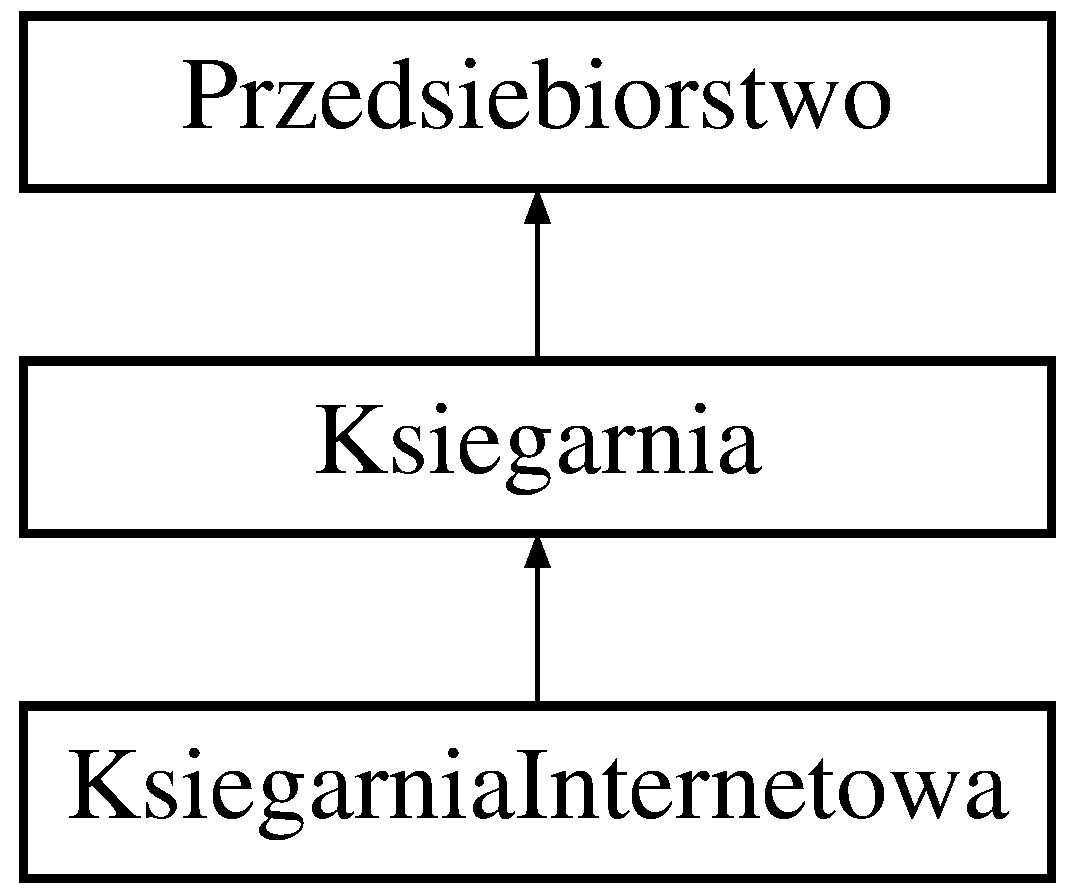
\includegraphics[height=3.000000cm]{class_ksiegarnia_internetowa}
\end{center}
\end{figure}
\subsection*{Public Member Functions}
\begin{DoxyCompactItemize}
\item 
\textbf{ Ksiegarnia\+Internetowa} ()
\begin{DoxyCompactList}\small\item\em Konstruktor domyslny. \end{DoxyCompactList}\item 
\textbf{ $\sim$\+Ksiegarnia\+Internetowa} ()
\begin{DoxyCompactList}\small\item\em Destruktor. \end{DoxyCompactList}\item 
void \textbf{ wypisz\+Dane\+Firmy} (ostream \&s)
\begin{DoxyCompactList}\small\item\em Metoda pozwalajaca uzyskac dane na temat Ksiegarni Internetowej. \end{DoxyCompactList}\item 
void \textbf{ wprowadz\+Dane\+Firmy\+Z\+Pliku} (istream \&s)
\begin{DoxyCompactList}\small\item\em Metoda pozwalajaca na wprowadzenie danych Ksiegarni internetowej. \end{DoxyCompactList}\item 
void \textbf{ wprowadz\+Dane\+Ksiegarni\+Internetowej} (string nowy\+\_\+adres\+\_\+domeny)
\begin{DoxyCompactList}\small\item\em Metoda pozwalajaca wprowadzic dane Ksiegarni Internetowej. \end{DoxyCompactList}\end{DoxyCompactItemize}
\subsection*{Friends}
\begin{DoxyCompactItemize}
\item 
ostream \& \textbf{ operator$<$$<$} (ostream \&s, \textbf{ Ksiegarnia\+Internetowa} \&k)
\begin{DoxyCompactList}\small\item\em Zaprzyjazniony operator strumieniowy. \end{DoxyCompactList}\item 
istream \& \textbf{ operator$>$$>$} (istream \&s, \textbf{ Ksiegarnia\+Internetowa} \&k)
\begin{DoxyCompactList}\small\item\em Zaprzyjazniony operator strumieniowy. \end{DoxyCompactList}\end{DoxyCompactItemize}
\subsection*{Additional Inherited Members}


\subsection{Detailed Description}
Klasa \doxyref{Ksiegarnia}{p.}{class_ksiegarnia} Internetowa, pochodna klasy \doxyref{Ksiegarnia}{p.}{class_ksiegarnia}. 

\subsection{Constructor \& Destructor Documentation}
\mbox{\label{class_ksiegarnia_internetowa_ae33f7c87839ae4f0f39e8e4c697b00d3}} 
\index{Ksiegarnia\+Internetowa@{Ksiegarnia\+Internetowa}!Ksiegarnia\+Internetowa@{Ksiegarnia\+Internetowa}}
\index{Ksiegarnia\+Internetowa@{Ksiegarnia\+Internetowa}!Ksiegarnia\+Internetowa@{Ksiegarnia\+Internetowa}}
\subsubsection{Ksiegarnia\+Internetowa()}
{\footnotesize\ttfamily Ksiegarnia\+Internetowa\+::\+Ksiegarnia\+Internetowa (\begin{DoxyParamCaption}{ }\end{DoxyParamCaption})}



Konstruktor domyslny. 

Konstruktor domyslny obiektu \doxyref{Ksiegarnia}{p.}{class_ksiegarnia} internetowa. \mbox{\label{class_ksiegarnia_internetowa_a8e93f3b6b3d09d691bdea4084305c5de}} 
\index{Ksiegarnia\+Internetowa@{Ksiegarnia\+Internetowa}!````~Ksiegarnia\+Internetowa@{$\sim$\+Ksiegarnia\+Internetowa}}
\index{````~Ksiegarnia\+Internetowa@{$\sim$\+Ksiegarnia\+Internetowa}!Ksiegarnia\+Internetowa@{Ksiegarnia\+Internetowa}}
\subsubsection{$\sim$\+Ksiegarnia\+Internetowa()}
{\footnotesize\ttfamily Ksiegarnia\+Internetowa\+::$\sim$\+Ksiegarnia\+Internetowa (\begin{DoxyParamCaption}{ }\end{DoxyParamCaption})}



Destruktor. 



\subsection{Member Function Documentation}
\mbox{\label{class_ksiegarnia_internetowa_a9faf7af01f7dcfbab38f5e45f53ad269}} 
\index{Ksiegarnia\+Internetowa@{Ksiegarnia\+Internetowa}!wprowadz\+Dane\+Firmy\+Z\+Pliku@{wprowadz\+Dane\+Firmy\+Z\+Pliku}}
\index{wprowadz\+Dane\+Firmy\+Z\+Pliku@{wprowadz\+Dane\+Firmy\+Z\+Pliku}!Ksiegarnia\+Internetowa@{Ksiegarnia\+Internetowa}}
\subsubsection{wprowadz\+Dane\+Firmy\+Z\+Pliku()}
{\footnotesize\ttfamily void Ksiegarnia\+Internetowa\+::wprowadz\+Dane\+Firmy\+Z\+Pliku (\begin{DoxyParamCaption}\item[{istream \&}]{s }\end{DoxyParamCaption})\hspace{0.3cm}{\ttfamily [virtual]}}



Metoda pozwalajaca na wprowadzenie danych Ksiegarni internetowej. 

Umozliwia wprowadzanie danych obiektu z pliku. 

Reimplemented from \textbf{ Przedsiebiorstwo} \doxyref{}{p.}{class_przedsiebiorstwo_adff311023ef04e492b6a7db7d4a8a01c}.

\mbox{\label{class_ksiegarnia_internetowa_aaeffb133e8bff411f9751e35c23faff0}} 
\index{Ksiegarnia\+Internetowa@{Ksiegarnia\+Internetowa}!wprowadz\+Dane\+Ksiegarni\+Internetowej@{wprowadz\+Dane\+Ksiegarni\+Internetowej}}
\index{wprowadz\+Dane\+Ksiegarni\+Internetowej@{wprowadz\+Dane\+Ksiegarni\+Internetowej}!Ksiegarnia\+Internetowa@{Ksiegarnia\+Internetowa}}
\subsubsection{wprowadz\+Dane\+Ksiegarni\+Internetowej()}
{\footnotesize\ttfamily void Ksiegarnia\+Internetowa\+::wprowadz\+Dane\+Ksiegarni\+Internetowej (\begin{DoxyParamCaption}\item[{string}]{nowy\+\_\+adres\+\_\+domeny }\end{DoxyParamCaption})}



Metoda pozwalajaca wprowadzic dane Ksiegarni Internetowej. 

Metoda pozwala na dodanie adresu domeny Ksiegarni Internetowej. 
\begin{DoxyParams}{Parameters}
{\em nowy\+\_\+adres\+\_\+domeny} & adres domeny Ksiegarni Internetowej \\
\hline
\end{DoxyParams}
\mbox{\label{class_ksiegarnia_internetowa_aecf96702408f147af4414a5756beea59}} 
\index{Ksiegarnia\+Internetowa@{Ksiegarnia\+Internetowa}!wypisz\+Dane\+Firmy@{wypisz\+Dane\+Firmy}}
\index{wypisz\+Dane\+Firmy@{wypisz\+Dane\+Firmy}!Ksiegarnia\+Internetowa@{Ksiegarnia\+Internetowa}}
\subsubsection{wypisz\+Dane\+Firmy()}
{\footnotesize\ttfamily void Ksiegarnia\+Internetowa\+::wypisz\+Dane\+Firmy (\begin{DoxyParamCaption}\item[{ostream \&}]{s }\end{DoxyParamCaption})\hspace{0.3cm}{\ttfamily [virtual]}}



Metoda pozwalajaca uzyskac dane na temat Ksiegarni Internetowej. 

Umozliwia wyprowadzenie danych obiektu na dowolny strumien wyjscia. 
\begin{DoxyParams}{Parameters}
{\em s} & dowolny strumien wyjscia \\
\hline
\end{DoxyParams}


Implements \textbf{ Przedsiebiorstwo} \doxyref{}{p.}{class_przedsiebiorstwo_aff6ca5801f0160b5201be2209c58459d}.



\subsection{Friends And Related Function Documentation}
\mbox{\label{class_ksiegarnia_internetowa_acbed3e5b8b7c750fb018937826d93955}} 
\index{Ksiegarnia\+Internetowa@{Ksiegarnia\+Internetowa}!operator$<$$<$@{operator$<$$<$}}
\index{operator$<$$<$@{operator$<$$<$}!Ksiegarnia\+Internetowa@{Ksiegarnia\+Internetowa}}
\subsubsection{operator$<$$<$}
{\footnotesize\ttfamily ostream\& operator$<$$<$ (\begin{DoxyParamCaption}\item[{ostream \&}]{s,  }\item[{\textbf{ Ksiegarnia\+Internetowa} \&}]{k }\end{DoxyParamCaption})\hspace{0.3cm}{\ttfamily [friend]}}



Zaprzyjazniony operator strumieniowy. 

Przeciazony operator pozwala na uzyskanie danych na dowlny strumien wyjscia. W tym programie wykorzystywany do wypisu danych na standardowe wyjscie lub do pliku. \mbox{\label{class_ksiegarnia_internetowa_a7d80d3814dfd9ebbef98fd6de3aa46b5}} 
\index{Ksiegarnia\+Internetowa@{Ksiegarnia\+Internetowa}!operator$>$$>$@{operator$>$$>$}}
\index{operator$>$$>$@{operator$>$$>$}!Ksiegarnia\+Internetowa@{Ksiegarnia\+Internetowa}}
\subsubsection{operator$>$$>$}
{\footnotesize\ttfamily istream\& operator$>$$>$ (\begin{DoxyParamCaption}\item[{istream \&}]{s,  }\item[{\textbf{ Ksiegarnia\+Internetowa} \&}]{k }\end{DoxyParamCaption})\hspace{0.3cm}{\ttfamily [friend]}}



Zaprzyjazniony operator strumieniowy. 

Przeciazony operator pozwala na pobranie danych z dowolnego strumienia wejscia. W tym programie wykorzystywany do odczytu danych z pliku. 

The documentation for this class was generated from the following files\+:\begin{DoxyCompactItemize}
\item 
\textbf{ Ksiegarnia internetowa.\+h}\item 
\textbf{ Ksiegarnia internetowa.\+cpp}\end{DoxyCompactItemize}

\section{Pracownicy Class Reference}
\label{class_pracownicy}\index{Pracownicy@{Pracownicy}}


Klasa przechowujaca dane o pracownikach firmy.  




{\ttfamily \#include $<$Pracownicy.\+h$>$}

\subsection*{Public Member Functions}
\begin{DoxyCompactItemize}
\item 
\textbf{ Pracownicy} ()
\begin{DoxyCompactList}\small\item\em Konstruktor. \end{DoxyCompactList}\item 
\textbf{ Pracownicy} (string nowe\+\_\+nazw, float nowe\+\_\+zarob)
\begin{DoxyCompactList}\small\item\em Konstruktor z parametrami. \end{DoxyCompactList}\item 
\textbf{ $\sim$\+Pracownicy} ()
\begin{DoxyCompactList}\small\item\em Destruktor. \end{DoxyCompactList}\end{DoxyCompactItemize}
\subsection*{Friends}
\begin{DoxyCompactItemize}
\item 
ostream \& \textbf{ operator$<$$<$} (ostream \&s, \textbf{ Pracownicy} \&p)
\begin{DoxyCompactList}\small\item\em Zaprzyjazniony operator strumieniowy. \end{DoxyCompactList}\end{DoxyCompactItemize}


\subsection{Detailed Description}
Klasa przechowujaca dane o pracownikach firmy. 

\subsection{Constructor \& Destructor Documentation}
\mbox{\label{class_pracownicy_a4b6c44961abc642567c50d14ccededd8}} 
\index{Pracownicy@{Pracownicy}!Pracownicy@{Pracownicy}}
\index{Pracownicy@{Pracownicy}!Pracownicy@{Pracownicy}}
\subsubsection{Pracownicy()\hspace{0.1cm}{\footnotesize\ttfamily [1/2]}}
{\footnotesize\ttfamily Pracownicy\+::\+Pracownicy (\begin{DoxyParamCaption}{ }\end{DoxyParamCaption})}



Konstruktor. 

\mbox{\label{class_pracownicy_a274fe5e34de172af59b55f02bc9feead}} 
\index{Pracownicy@{Pracownicy}!Pracownicy@{Pracownicy}}
\index{Pracownicy@{Pracownicy}!Pracownicy@{Pracownicy}}
\subsubsection{Pracownicy()\hspace{0.1cm}{\footnotesize\ttfamily [2/2]}}
{\footnotesize\ttfamily Pracownicy\+::\+Pracownicy (\begin{DoxyParamCaption}\item[{string}]{nowe\+\_\+nazw,  }\item[{float}]{nowe\+\_\+zarob }\end{DoxyParamCaption})}



Konstruktor z parametrami. 

\mbox{\label{class_pracownicy_a712918bfaf884baaadaf5eca3aa131c1}} 
\index{Pracownicy@{Pracownicy}!````~Pracownicy@{$\sim$\+Pracownicy}}
\index{````~Pracownicy@{$\sim$\+Pracownicy}!Pracownicy@{Pracownicy}}
\subsubsection{$\sim$\+Pracownicy()}
{\footnotesize\ttfamily Pracownicy\+::$\sim$\+Pracownicy (\begin{DoxyParamCaption}{ }\end{DoxyParamCaption})}



Destruktor. 



\subsection{Friends And Related Function Documentation}
\mbox{\label{class_pracownicy_a982680671c2057a272ee1ab713a2fc5f}} 
\index{Pracownicy@{Pracownicy}!operator$<$$<$@{operator$<$$<$}}
\index{operator$<$$<$@{operator$<$$<$}!Pracownicy@{Pracownicy}}
\subsubsection{operator$<$$<$}
{\footnotesize\ttfamily ostream\& operator$<$$<$ (\begin{DoxyParamCaption}\item[{ostream \&}]{s,  }\item[{\textbf{ Pracownicy} \&}]{p }\end{DoxyParamCaption})\hspace{0.3cm}{\ttfamily [friend]}}



Zaprzyjazniony operator strumieniowy. 

Przeciazony operator pozwala na uzyskanie danych na dowolny strumien wyjscia. W tym programie wykorzystywany do wypisu danych na standardowe wyjscie lub do pliku. 

The documentation for this class was generated from the following files\+:\begin{DoxyCompactItemize}
\item 
\textbf{ Pracownicy.\+h}\item 
\textbf{ Pracownicy.\+cpp}\end{DoxyCompactItemize}

\section{Przedsiebiorstwo Class Reference}
\label{class_przedsiebiorstwo}\index{Przedsiebiorstwo@{Przedsiebiorstwo}}


Klasa abstrakcyjna.  




{\ttfamily \#include $<$Przedsiebiorstwo.\+h$>$}

Inheritance diagram for Przedsiebiorstwo\+:\begin{figure}[H]
\begin{center}
\leavevmode
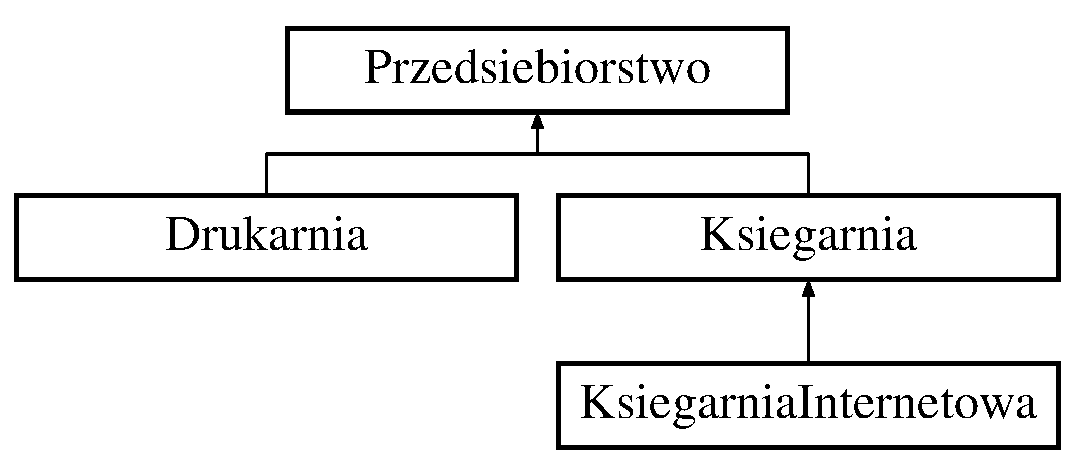
\includegraphics[height=3.000000cm]{class_przedsiebiorstwo}
\end{center}
\end{figure}
\subsection*{Public Member Functions}
\begin{DoxyCompactItemize}
\item 
\textbf{ Przedsiebiorstwo} ()
\begin{DoxyCompactList}\small\item\em Kontruktor domyslny. \end{DoxyCompactList}\item 
virtual \textbf{ $\sim$\+Przedsiebiorstwo} ()
\begin{DoxyCompactList}\small\item\em Destruktor wirtualny. \end{DoxyCompactList}\item 
virtual void \textbf{ wypisz\+Dane\+Firmy} (ostream \&s)=0
\begin{DoxyCompactList}\small\item\em Metoda abstrakcyjna pozwalajaca uzyskac dane klas pochodnych. \end{DoxyCompactList}\item 
virtual void \textbf{ wprowadz\+Dane\+Firmy\+Z\+Pliku} (istream \&s)
\begin{DoxyCompactList}\small\item\em Metoda abstrakcyjna pozwalajaca na wprowadzenie danych utworzonego obiektu. \end{DoxyCompactList}\item 
void \textbf{ wypisz\+Glowne\+Dane\+Firmy} (ostream \&s)
\begin{DoxyCompactList}\small\item\em Metoda pozwalajaca uzyskac dane klasy podstawowej. \end{DoxyCompactList}\item 
void \textbf{ wprowadz\+Dane\+Przedsiebiorstwa} (string nowa\+\_\+nazwa, string nowy\+\_\+wlasciciel)
\begin{DoxyCompactList}\small\item\em Metoda pozwalajaca wprowadzic dane przedsiebiorstwa. \end{DoxyCompactList}\item 
void \textbf{ dodaj\+Pracownika} (string nazwisko, float zarobki)
\begin{DoxyCompactList}\small\item\em Metoda pozwalajaca dodac pracownika do przedsiebiorstwa. \end{DoxyCompactList}\item 
void \textbf{ usun\+Pracownika} (int ktory)
\begin{DoxyCompactList}\small\item\em Metoda pozwalajaca usunac pracownika z przedsiebiorstwa. \end{DoxyCompactList}\end{DoxyCompactItemize}
\subsection*{Protected Attributes}
\begin{DoxyCompactItemize}
\item 
string \textbf{ nazwa\+\_\+przedsiebiorstwa}
\begin{DoxyCompactList}\small\item\em zmienna przechowujaca nazwe przedsiebiorstwa \end{DoxyCompactList}\item 
string \textbf{ wlasciciel}
\begin{DoxyCompactList}\small\item\em zmienna przechowujaca imie i nazwisko wlasciciela \end{DoxyCompactList}\item 
vector$<$ \textbf{ Pracownicy} $>$ \textbf{ pracownicy}
\begin{DoxyCompactList}\small\item\em kontener zawierajacy dane pracownikow przedsiebiorstwa \end{DoxyCompactList}\item 
\textbf{ Siedziba} \textbf{ siedziba}
\begin{DoxyCompactList}\small\item\em siedziba klasa opisujaca siedziby firm wchodzacych w sklad przedsiebiorstwa \end{DoxyCompactList}\end{DoxyCompactItemize}
\subsection*{Static Protected Attributes}
\begin{DoxyCompactItemize}
\item 
static int \textbf{ ilosc\+Przedsiebiorstw} = 0
\begin{DoxyCompactList}\small\item\em zmienna przechowujaca ilosc utworzonych obiektow (Przedsiebiorstw) \end{DoxyCompactList}\end{DoxyCompactItemize}
\subsection*{Friends}
\begin{DoxyCompactItemize}
\item 
ostream \& \textbf{ operator$<$$<$} (ostream \&s, \textbf{ Przedsiebiorstwo} \&p)
\begin{DoxyCompactList}\small\item\em Operator strumieniowy $<$$<$. \end{DoxyCompactList}\item 
istream \& \textbf{ operator$>$$>$} (istream \&s, \textbf{ Przedsiebiorstwo} \&p)
\begin{DoxyCompactList}\small\item\em Operator strumieniowy $>$$>$ \end{DoxyCompactList}\end{DoxyCompactItemize}


\subsection{Detailed Description}
Klasa abstrakcyjna. 

\subsection{Constructor \& Destructor Documentation}
\mbox{\label{class_przedsiebiorstwo_ab6500b19c5689f5dd77f033ff66dcf75}} 
\index{Przedsiebiorstwo@{Przedsiebiorstwo}!Przedsiebiorstwo@{Przedsiebiorstwo}}
\index{Przedsiebiorstwo@{Przedsiebiorstwo}!Przedsiebiorstwo@{Przedsiebiorstwo}}
\subsubsection{Przedsiebiorstwo()}
{\footnotesize\ttfamily Przedsiebiorstwo\+::\+Przedsiebiorstwo (\begin{DoxyParamCaption}{ }\end{DoxyParamCaption})}



Kontruktor domyslny. 

\mbox{\label{class_przedsiebiorstwo_a760b0930bdcefffbb78837026d5cd506}} 
\index{Przedsiebiorstwo@{Przedsiebiorstwo}!````~Przedsiebiorstwo@{$\sim$\+Przedsiebiorstwo}}
\index{````~Przedsiebiorstwo@{$\sim$\+Przedsiebiorstwo}!Przedsiebiorstwo@{Przedsiebiorstwo}}
\subsubsection{$\sim$\+Przedsiebiorstwo()}
{\footnotesize\ttfamily Przedsiebiorstwo\+::$\sim$\+Przedsiebiorstwo (\begin{DoxyParamCaption}{ }\end{DoxyParamCaption})\hspace{0.3cm}{\ttfamily [virtual]}}



Destruktor wirtualny. 



\subsection{Member Function Documentation}
\mbox{\label{class_przedsiebiorstwo_a72e22097469dbf897f47307ec957b1f1}} 
\index{Przedsiebiorstwo@{Przedsiebiorstwo}!dodaj\+Pracownika@{dodaj\+Pracownika}}
\index{dodaj\+Pracownika@{dodaj\+Pracownika}!Przedsiebiorstwo@{Przedsiebiorstwo}}
\subsubsection{dodaj\+Pracownika()}
{\footnotesize\ttfamily void Przedsiebiorstwo\+::dodaj\+Pracownika (\begin{DoxyParamCaption}\item[{string}]{nazwisko,  }\item[{float}]{zarobki }\end{DoxyParamCaption})}



Metoda pozwalajaca dodac pracownika do przedsiebiorstwa. 

Metoda pozwala na dodanie pracownika o podanym nazwisku i zarobkach. 
\begin{DoxyParams}{Parameters}
{\em nazwisko} & nazwisko pracownika ktorego chcemy dodac do firmy \\
\hline
{\em zarobki} & zarobki pracownika ktorego chcemy dodac do firmy \\
\hline
\end{DoxyParams}
\mbox{\label{class_przedsiebiorstwo_a376e3d39d574bef0eea6b906c379d502}} 
\index{Przedsiebiorstwo@{Przedsiebiorstwo}!usun\+Pracownika@{usun\+Pracownika}}
\index{usun\+Pracownika@{usun\+Pracownika}!Przedsiebiorstwo@{Przedsiebiorstwo}}
\subsubsection{usun\+Pracownika()}
{\footnotesize\ttfamily void Przedsiebiorstwo\+::usun\+Pracownika (\begin{DoxyParamCaption}\item[{int}]{ktory }\end{DoxyParamCaption})}



Metoda pozwalajaca usunac pracownika z przedsiebiorstwa. 

Metoda pozwala na usuniecie pracownika o wybranym numerze. 
\begin{DoxyParams}{Parameters}
{\em ktory} & numer pracownika ktorego chcemy usunac z firmy \\
\hline
\end{DoxyParams}
\mbox{\label{class_przedsiebiorstwo_adff311023ef04e492b6a7db7d4a8a01c}} 
\index{Przedsiebiorstwo@{Przedsiebiorstwo}!wprowadz\+Dane\+Firmy\+Z\+Pliku@{wprowadz\+Dane\+Firmy\+Z\+Pliku}}
\index{wprowadz\+Dane\+Firmy\+Z\+Pliku@{wprowadz\+Dane\+Firmy\+Z\+Pliku}!Przedsiebiorstwo@{Przedsiebiorstwo}}
\subsubsection{wprowadz\+Dane\+Firmy\+Z\+Pliku()}
{\footnotesize\ttfamily void Przedsiebiorstwo\+::wprowadz\+Dane\+Firmy\+Z\+Pliku (\begin{DoxyParamCaption}\item[{istream \&}]{s }\end{DoxyParamCaption})\hspace{0.3cm}{\ttfamily [virtual]}}



Metoda abstrakcyjna pozwalajaca na wprowadzenie danych utworzonego obiektu. 

Umozliwia wprowadzanie danych obiektu z pliku. 
\begin{DoxyParams}{Parameters}
{\em s} & strumien wejscia \\
\hline
\end{DoxyParams}


Reimplemented in \textbf{ Ksiegarnia} \doxyref{}{p.}{class_ksiegarnia_a6fb5c23404419a9f2e2fb345e2c28289}, \textbf{ Drukarnia} \doxyref{}{p.}{class_drukarnia_aa77de3fe83557754ebac4a6b4a443c9d}, and \textbf{ Ksiegarnia\+Internetowa} \doxyref{}{p.}{class_ksiegarnia_internetowa_a9faf7af01f7dcfbab38f5e45f53ad269}.

\mbox{\label{class_przedsiebiorstwo_abe2e14ce98477bbc26d0493496ab975f}} 
\index{Przedsiebiorstwo@{Przedsiebiorstwo}!wprowadz\+Dane\+Przedsiebiorstwa@{wprowadz\+Dane\+Przedsiebiorstwa}}
\index{wprowadz\+Dane\+Przedsiebiorstwa@{wprowadz\+Dane\+Przedsiebiorstwa}!Przedsiebiorstwo@{Przedsiebiorstwo}}
\subsubsection{wprowadz\+Dane\+Przedsiebiorstwa()}
{\footnotesize\ttfamily void Przedsiebiorstwo\+::wprowadz\+Dane\+Przedsiebiorstwa (\begin{DoxyParamCaption}\item[{string}]{nowa\+\_\+nazwa,  }\item[{string}]{nowy\+\_\+wlasciciel }\end{DoxyParamCaption})}



Metoda pozwalajaca wprowadzic dane przedsiebiorstwa. 

Metoda pozwala na dodanie nazwy i wlasciciela firmy. 
\begin{DoxyParams}{Parameters}
{\em nowa\+\_\+nazwa} & nazwa przedsiebiorstwa \\
\hline
{\em nowy\+\_\+wlasciciel} & imie i nazwisko wlasciciela przedsiebiorstwa \\
\hline
\end{DoxyParams}
\mbox{\label{class_przedsiebiorstwo_aff6ca5801f0160b5201be2209c58459d}} 
\index{Przedsiebiorstwo@{Przedsiebiorstwo}!wypisz\+Dane\+Firmy@{wypisz\+Dane\+Firmy}}
\index{wypisz\+Dane\+Firmy@{wypisz\+Dane\+Firmy}!Przedsiebiorstwo@{Przedsiebiorstwo}}
\subsubsection{wypisz\+Dane\+Firmy()}
{\footnotesize\ttfamily virtual void Przedsiebiorstwo\+::wypisz\+Dane\+Firmy (\begin{DoxyParamCaption}\item[{ostream \&}]{s }\end{DoxyParamCaption})\hspace{0.3cm}{\ttfamily [pure virtual]}}



Metoda abstrakcyjna pozwalajaca uzyskac dane klas pochodnych. 

Umozliwia wyprowadzenie danych obiektu na dowolny strumien wyjscia. 
\begin{DoxyParams}{Parameters}
{\em s} & dowolny strumien wyjscia \\
\hline
\end{DoxyParams}


Implemented in \textbf{ Ksiegarnia} \doxyref{}{p.}{class_ksiegarnia_a106be862cec81c42fe742ddfc9f60768}, \textbf{ Drukarnia} \doxyref{}{p.}{class_drukarnia_a9ebed3c69bdb7fbc30dfca3fda086233}, and \textbf{ Ksiegarnia\+Internetowa} \doxyref{}{p.}{class_ksiegarnia_internetowa_aecf96702408f147af4414a5756beea59}.

\mbox{\label{class_przedsiebiorstwo_a266ab2a1663cfc0767c062e38a2a4fc7}} 
\index{Przedsiebiorstwo@{Przedsiebiorstwo}!wypisz\+Glowne\+Dane\+Firmy@{wypisz\+Glowne\+Dane\+Firmy}}
\index{wypisz\+Glowne\+Dane\+Firmy@{wypisz\+Glowne\+Dane\+Firmy}!Przedsiebiorstwo@{Przedsiebiorstwo}}
\subsubsection{wypisz\+Glowne\+Dane\+Firmy()}
{\footnotesize\ttfamily void Przedsiebiorstwo\+::wypisz\+Glowne\+Dane\+Firmy (\begin{DoxyParamCaption}\item[{ostream \&}]{s }\end{DoxyParamCaption})}



Metoda pozwalajaca uzyskac dane klasy podstawowej. 

Umozliwia wyprowadzenie danych obiektu na dowolny strumien wyjscia. 
\begin{DoxyParams}{Parameters}
{\em s} & dowolny strumien wyjscia \\
\hline
\end{DoxyParams}


\subsection{Friends And Related Function Documentation}
\mbox{\label{class_przedsiebiorstwo_a1c4af9010b5f2325f11a349a702c78ef}} 
\index{Przedsiebiorstwo@{Przedsiebiorstwo}!operator$<$$<$@{operator$<$$<$}}
\index{operator$<$$<$@{operator$<$$<$}!Przedsiebiorstwo@{Przedsiebiorstwo}}
\subsubsection{operator$<$$<$}
{\footnotesize\ttfamily ostream\& operator$<$$<$ (\begin{DoxyParamCaption}\item[{ostream \&}]{s,  }\item[{\textbf{ Przedsiebiorstwo} \&}]{p }\end{DoxyParamCaption})\hspace{0.3cm}{\ttfamily [friend]}}



Operator strumieniowy $<$$<$. 

Przeciazony operator pozwala na uzyskanie danych na dowlny strumien wyjscia. W tym programie wykorzystywany do wypisu danych na standardowe wyjscie lub do pliku. \mbox{\label{class_przedsiebiorstwo_af9de6edea9cbaa7152816ed3251f934e}} 
\index{Przedsiebiorstwo@{Przedsiebiorstwo}!operator$>$$>$@{operator$>$$>$}}
\index{operator$>$$>$@{operator$>$$>$}!Przedsiebiorstwo@{Przedsiebiorstwo}}
\subsubsection{operator$>$$>$}
{\footnotesize\ttfamily istream\& operator$>$$>$ (\begin{DoxyParamCaption}\item[{istream \&}]{s,  }\item[{\textbf{ Przedsiebiorstwo} \&}]{p }\end{DoxyParamCaption})\hspace{0.3cm}{\ttfamily [friend]}}



Operator strumieniowy $>$$>$ 

Przeciazony operator pozwala na pobranie danych z dowolnego strumienia wejscia. W tym programie wykorzystywany do odczytu danych z pliku. 

\subsection{Member Data Documentation}
\mbox{\label{class_przedsiebiorstwo_aac6039457106a22c6b889115d4381c8e}} 
\index{Przedsiebiorstwo@{Przedsiebiorstwo}!ilosc\+Przedsiebiorstw@{ilosc\+Przedsiebiorstw}}
\index{ilosc\+Przedsiebiorstw@{ilosc\+Przedsiebiorstw}!Przedsiebiorstwo@{Przedsiebiorstwo}}
\subsubsection{ilosc\+Przedsiebiorstw}
{\footnotesize\ttfamily int Przedsiebiorstwo\+::ilosc\+Przedsiebiorstw = 0\hspace{0.3cm}{\ttfamily [static]}, {\ttfamily [protected]}}



zmienna przechowujaca ilosc utworzonych obiektow (Przedsiebiorstw) 

\mbox{\label{class_przedsiebiorstwo_acbbb2c4e2480dba4edd227a136175644}} 
\index{Przedsiebiorstwo@{Przedsiebiorstwo}!nazwa\+\_\+przedsiebiorstwa@{nazwa\+\_\+przedsiebiorstwa}}
\index{nazwa\+\_\+przedsiebiorstwa@{nazwa\+\_\+przedsiebiorstwa}!Przedsiebiorstwo@{Przedsiebiorstwo}}
\subsubsection{nazwa\+\_\+przedsiebiorstwa}
{\footnotesize\ttfamily string Przedsiebiorstwo\+::nazwa\+\_\+przedsiebiorstwa\hspace{0.3cm}{\ttfamily [protected]}}



zmienna przechowujaca nazwe przedsiebiorstwa 

\mbox{\label{class_przedsiebiorstwo_a263daafed00961aafa077d00e7180216}} 
\index{Przedsiebiorstwo@{Przedsiebiorstwo}!pracownicy@{pracownicy}}
\index{pracownicy@{pracownicy}!Przedsiebiorstwo@{Przedsiebiorstwo}}
\subsubsection{pracownicy}
{\footnotesize\ttfamily vector$<$\textbf{ Pracownicy}$>$ Przedsiebiorstwo\+::pracownicy\hspace{0.3cm}{\ttfamily [protected]}}



kontener zawierajacy dane pracownikow przedsiebiorstwa 

\mbox{\label{class_przedsiebiorstwo_a584172e3ca0457865c21b85318a7824e}} 
\index{Przedsiebiorstwo@{Przedsiebiorstwo}!siedziba@{siedziba}}
\index{siedziba@{siedziba}!Przedsiebiorstwo@{Przedsiebiorstwo}}
\subsubsection{siedziba}
{\footnotesize\ttfamily \textbf{ Siedziba} Przedsiebiorstwo\+::siedziba\hspace{0.3cm}{\ttfamily [protected]}}



siedziba klasa opisujaca siedziby firm wchodzacych w sklad przedsiebiorstwa 

\mbox{\label{class_przedsiebiorstwo_a8ef85eb78779d8b3fe11d9b24a9fdcf1}} 
\index{Przedsiebiorstwo@{Przedsiebiorstwo}!wlasciciel@{wlasciciel}}
\index{wlasciciel@{wlasciciel}!Przedsiebiorstwo@{Przedsiebiorstwo}}
\subsubsection{wlasciciel}
{\footnotesize\ttfamily string Przedsiebiorstwo\+::wlasciciel\hspace{0.3cm}{\ttfamily [protected]}}



zmienna przechowujaca imie i nazwisko wlasciciela 



The documentation for this class was generated from the following files\+:\begin{DoxyCompactItemize}
\item 
\textbf{ Przedsiebiorstwo.\+h}\item 
\textbf{ Przedsiebiorstwo.\+cpp}\end{DoxyCompactItemize}

\section{Siedziba Class Reference}
\label{class_siedziba}\index{Siedziba@{Siedziba}}


Klasa przechowujaca dane o siedzibie firmy.  




{\ttfamily \#include $<$Siedziba.\+h$>$}

\subsection*{Public Member Functions}
\begin{DoxyCompactItemize}
\item 
void \textbf{ wypisz\+Siedzibe} (ostream \&s)
\begin{DoxyCompactList}\small\item\em Metoda pozwalajaca wyswietlic siedzibe firmy. \end{DoxyCompactList}\item 
\textbf{ Siedziba} ()
\begin{DoxyCompactList}\small\item\em Konstruktor domyslny. \end{DoxyCompactList}\item 
void \textbf{ ustaw\+Dane\+Siedziby} (string nowy\+\_\+adres, int nowy\+\_\+numer)
\begin{DoxyCompactList}\small\item\em Metoda pozwalajaca ustawic dane Siedziby. \end{DoxyCompactList}\item 
\textbf{ $\sim$\+Siedziba} ()
\begin{DoxyCompactList}\small\item\em Destruktor. \end{DoxyCompactList}\end{DoxyCompactItemize}
\subsection*{Friends}
\begin{DoxyCompactItemize}
\item 
istream \& \textbf{ operator$>$$>$} (istream \&s, \textbf{ Siedziba} \&sb)
\begin{DoxyCompactList}\small\item\em Zaprzyjazniony operator strumieniowy. \end{DoxyCompactList}\item 
ostream \& \textbf{ operator$<$$<$} (ostream \&s, \textbf{ Siedziba} \&sb)
\begin{DoxyCompactList}\small\item\em Zaprzyjazniony operator strumieniowy. \end{DoxyCompactList}\end{DoxyCompactItemize}


\subsection{Detailed Description}
Klasa przechowujaca dane o siedzibie firmy. 

\subsection{Constructor \& Destructor Documentation}
\mbox{\label{class_siedziba_a3d2babb95b8eae60c04eb73c9db0981c}} 
\index{Siedziba@{Siedziba}!Siedziba@{Siedziba}}
\index{Siedziba@{Siedziba}!Siedziba@{Siedziba}}
\subsubsection{Siedziba()}
{\footnotesize\ttfamily Siedziba\+::\+Siedziba (\begin{DoxyParamCaption}{ }\end{DoxyParamCaption})}



Konstruktor domyslny. 

\mbox{\label{class_siedziba_a1dc3fee9549a390981000aa8df28ee1e}} 
\index{Siedziba@{Siedziba}!````~Siedziba@{$\sim$\+Siedziba}}
\index{````~Siedziba@{$\sim$\+Siedziba}!Siedziba@{Siedziba}}
\subsubsection{$\sim$\+Siedziba()}
{\footnotesize\ttfamily Siedziba\+::$\sim$\+Siedziba (\begin{DoxyParamCaption}{ }\end{DoxyParamCaption})}



Destruktor. 



\subsection{Member Function Documentation}
\mbox{\label{class_siedziba_a43a381bfd9f56e65174998606f3919c4}} 
\index{Siedziba@{Siedziba}!ustaw\+Dane\+Siedziby@{ustaw\+Dane\+Siedziby}}
\index{ustaw\+Dane\+Siedziby@{ustaw\+Dane\+Siedziby}!Siedziba@{Siedziba}}
\subsubsection{ustaw\+Dane\+Siedziby()}
{\footnotesize\ttfamily void Siedziba\+::ustaw\+Dane\+Siedziby (\begin{DoxyParamCaption}\item[{string}]{nowy\+\_\+adres,  }\item[{int}]{nowy\+\_\+numer }\end{DoxyParamCaption})}



Metoda pozwalajaca ustawic dane Siedziby. 

Metoda pozwala na ustawienie danych siedziby firmy. 
\begin{DoxyParams}{Parameters}
{\em nowy\+\_\+adres} & adres firmy \\
\hline
{\em nowy\+\_\+numer} & numer telefonu do firmy \\
\hline
\end{DoxyParams}
\mbox{\label{class_siedziba_a6f88b7a631efa99b8203154338d79c55}} 
\index{Siedziba@{Siedziba}!wypisz\+Siedzibe@{wypisz\+Siedzibe}}
\index{wypisz\+Siedzibe@{wypisz\+Siedzibe}!Siedziba@{Siedziba}}
\subsubsection{wypisz\+Siedzibe()}
{\footnotesize\ttfamily void Siedziba\+::wypisz\+Siedzibe (\begin{DoxyParamCaption}\item[{ostream \&}]{s }\end{DoxyParamCaption})}



Metoda pozwalajaca wyswietlic siedzibe firmy. 

Metoda umozliwia wyprowadzenie danych obiektu na dowolny strumien wyjscia. 
\begin{DoxyParams}{Parameters}
{\em s} & dowolny strumien wyjscia \\
\hline
\end{DoxyParams}


\subsection{Friends And Related Function Documentation}
\mbox{\label{class_siedziba_a9f6b107d8d81cef2e0ed0a865b1790f9}} 
\index{Siedziba@{Siedziba}!operator$<$$<$@{operator$<$$<$}}
\index{operator$<$$<$@{operator$<$$<$}!Siedziba@{Siedziba}}
\subsubsection{operator$<$$<$}
{\footnotesize\ttfamily ostream\& operator$<$$<$ (\begin{DoxyParamCaption}\item[{ostream \&}]{s,  }\item[{\textbf{ Siedziba} \&}]{sb }\end{DoxyParamCaption})\hspace{0.3cm}{\ttfamily [friend]}}



Zaprzyjazniony operator strumieniowy. 

Przeciazony operator pozwala na uzyskanie danych na dowlny strumien wyjscia. W tym programie wykorzystywany do wypisu danych na standardowe wyjscie lub do pliku. \mbox{\label{class_siedziba_ae5ef581c1d198741a15a44ad17c0960b}} 
\index{Siedziba@{Siedziba}!operator$>$$>$@{operator$>$$>$}}
\index{operator$>$$>$@{operator$>$$>$}!Siedziba@{Siedziba}}
\subsubsection{operator$>$$>$}
{\footnotesize\ttfamily istream\& operator$>$$>$ (\begin{DoxyParamCaption}\item[{istream \&}]{s,  }\item[{\textbf{ Siedziba} \&}]{sb }\end{DoxyParamCaption})\hspace{0.3cm}{\ttfamily [friend]}}



Zaprzyjazniony operator strumieniowy. 

Przeciazony operator pozwala na pobranie danych z dowolnego strumienia wejscia. W tym programie wykorzystywany do odczytu danych z pliku. 

The documentation for this class was generated from the following files\+:\begin{DoxyCompactItemize}
\item 
\textbf{ Siedziba.\+h}\item 
\textbf{ Siedziba.\+cpp}\end{DoxyCompactItemize}

\chapter{File Documentation}
\section{Drukarnia.\+cpp File Reference}
\label{_drukarnia_8cpp}\index{Drukarnia.\+cpp@{Drukarnia.\+cpp}}
{\ttfamily \#include $<$iostream$>$}\newline
{\ttfamily \#include $<$string$>$}\newline
{\ttfamily \#include \char`\"{}Drukarnia.\+h\char`\"{}}\newline
\subsection*{Functions}
\begin{DoxyCompactItemize}
\item 
ostream \& \textbf{ operator$<$$<$} (ostream \&s, \textbf{ Drukarnia} \&d)
\begin{DoxyCompactList}\small\item\em Przeciazony operator wyjscia. \end{DoxyCompactList}\item 
istream \& \textbf{ operator$>$$>$} (istream \&s, \textbf{ Drukarnia} \&d)
\begin{DoxyCompactList}\small\item\em Przeciazony operator wejscia. \end{DoxyCompactList}\end{DoxyCompactItemize}


\subsection{Function Documentation}
\mbox{\label{_drukarnia_8cpp_a0980f69a891e6b38b5bba72efa182ef9}} 
\index{Drukarnia.\+cpp@{Drukarnia.\+cpp}!operator$<$$<$@{operator$<$$<$}}
\index{operator$<$$<$@{operator$<$$<$}!Drukarnia.\+cpp@{Drukarnia.\+cpp}}
\subsubsection{operator$<$$<$()}
{\footnotesize\ttfamily ostream\& operator$<$$<$ (\begin{DoxyParamCaption}\item[{ostream \&}]{s,  }\item[{\textbf{ Drukarnia} \&}]{d }\end{DoxyParamCaption})}



Przeciazony operator wyjscia. 

Zaprzyjazniony operator strumieniowy.

Przeciazony operator pozwala na uzyskanie danych na dowlny strumien wyjscia. W tym programie wykorzystywany do wypisu danych na standardowe wyjscie lub do pliku. \mbox{\label{_drukarnia_8cpp_af4a4c25098d3c4c31f1f16d79bedeaa9}} 
\index{Drukarnia.\+cpp@{Drukarnia.\+cpp}!operator$>$$>$@{operator$>$$>$}}
\index{operator$>$$>$@{operator$>$$>$}!Drukarnia.\+cpp@{Drukarnia.\+cpp}}
\subsubsection{operator$>$$>$()}
{\footnotesize\ttfamily istream\& operator$>$$>$ (\begin{DoxyParamCaption}\item[{istream \&}]{s,  }\item[{\textbf{ Drukarnia} \&}]{d }\end{DoxyParamCaption})}



Przeciazony operator wejscia. 

Zaprzyjazniony operator strumieniowy.

Przeciazony operator pozwala na pobranie danych z dowolnego strumienia wejscia. W tym programie wykorzystywany do odczytu danych z pliku. 
\section{Drukarnia.\+h File Reference}
\label{_drukarnia_8h}\index{Drukarnia.\+h@{Drukarnia.\+h}}
{\ttfamily \#include $<$iostream$>$}\newline
{\ttfamily \#include $<$string$>$}\newline
{\ttfamily \#include $<$vector$>$}\newline
{\ttfamily \#include \char`\"{}Przedsiebiorstwo.\+h\char`\"{}}\newline
{\ttfamily \#include \char`\"{}Pracownicy.\+h\char`\"{}}\newline
{\ttfamily \#include \char`\"{}Siedziba.\+h\char`\"{}}\newline
\subsection*{Classes}
\begin{DoxyCompactItemize}
\item 
class \textbf{ Drukarnia}
\begin{DoxyCompactList}\small\item\em Klasa \doxyref{Drukarnia}{p.}{class_drukarnia}, pochodna klasy \doxyref{Przedsiebiorstwo}{p.}{class_przedsiebiorstwo}. \end{DoxyCompactList}\end{DoxyCompactItemize}
\subsection*{Functions}
\begin{DoxyCompactItemize}
\item 
istream \& \textbf{ operator$>$$>$} (istream \&s, \textbf{ Drukarnia} \&d)
\begin{DoxyCompactList}\small\item\em Przeciazony operator wejscia. \end{DoxyCompactList}\item 
ostream \& \textbf{ operator$<$$<$} (ostream \&s, \textbf{ Drukarnia} \&d)
\begin{DoxyCompactList}\small\item\em Przeciazony operator wyjscia. \end{DoxyCompactList}\end{DoxyCompactItemize}


\subsection{Function Documentation}
\mbox{\label{_drukarnia_8h_a0980f69a891e6b38b5bba72efa182ef9}} 
\index{Drukarnia.\+h@{Drukarnia.\+h}!operator$<$$<$@{operator$<$$<$}}
\index{operator$<$$<$@{operator$<$$<$}!Drukarnia.\+h@{Drukarnia.\+h}}
\subsubsection{operator$<$$<$()}
{\footnotesize\ttfamily ostream\& operator$<$$<$ (\begin{DoxyParamCaption}\item[{ostream \&}]{s,  }\item[{\textbf{ Drukarnia} \&}]{d }\end{DoxyParamCaption})}



Przeciazony operator wyjscia. 

Zaprzyjazniony operator strumieniowy.

Przeciazony operator pozwala na uzyskanie danych na dowlny strumien wyjscia. W tym programie wykorzystywany do wypisu danych na standardowe wyjscie lub do pliku. \mbox{\label{_drukarnia_8h_af4a4c25098d3c4c31f1f16d79bedeaa9}} 
\index{Drukarnia.\+h@{Drukarnia.\+h}!operator$>$$>$@{operator$>$$>$}}
\index{operator$>$$>$@{operator$>$$>$}!Drukarnia.\+h@{Drukarnia.\+h}}
\subsubsection{operator$>$$>$()}
{\footnotesize\ttfamily istream\& operator$>$$>$ (\begin{DoxyParamCaption}\item[{istream \&}]{s,  }\item[{\textbf{ Drukarnia} \&}]{d }\end{DoxyParamCaption})}



Przeciazony operator wejscia. 

Zaprzyjazniony operator strumieniowy.

Przeciazony operator pozwala na pobranie danych z dowolnego strumienia wejscia. W tym programie wykorzystywany do odczytu danych z pliku. 
\section{Ksiazka.\+cpp File Reference}
\label{_ksiazka_8cpp}\index{Ksiazka.\+cpp@{Ksiazka.\+cpp}}
{\ttfamily \#include $<$iostream$>$}\newline
{\ttfamily \#include $<$string$>$}\newline
{\ttfamily \#include \char`\"{}Ksiazka.\+h\char`\"{}}\newline
\subsection*{Functions}
\begin{DoxyCompactItemize}
\item 
ostream \& \textbf{ operator$<$$<$} (ostream \&s, \textbf{ Ksiazka} \&k)
\begin{DoxyCompactList}\small\item\em Przeciazony operator wyjscia. \end{DoxyCompactList}\end{DoxyCompactItemize}


\subsection{Function Documentation}
\mbox{\label{_ksiazka_8cpp_a6304f50ce62c067a686efe441f71c54d}} 
\index{Ksiazka.\+cpp@{Ksiazka.\+cpp}!operator$<$$<$@{operator$<$$<$}}
\index{operator$<$$<$@{operator$<$$<$}!Ksiazka.\+cpp@{Ksiazka.\+cpp}}
\subsubsection{operator$<$$<$()}
{\footnotesize\ttfamily ostream\& operator$<$$<$ (\begin{DoxyParamCaption}\item[{ostream \&}]{s,  }\item[{\textbf{ Ksiazka} \&}]{k }\end{DoxyParamCaption})}



Przeciazony operator wyjscia. 

Zaprzyjazniony operator strumieniowy.

Przeciazony operator pozwala na uzyskanie danych na dowolny strumien wyjscia. W tym programie wykorzystywany do wypisu danych na standardowe wyjscie lub do pliku. 
\section{Ksiazka.\+h File Reference}
\label{_ksiazka_8h}\index{Ksiazka.\+h@{Ksiazka.\+h}}
{\ttfamily \#include $<$iostream$>$}\newline
{\ttfamily \#include $<$string$>$}\newline
\subsection*{Classes}
\begin{DoxyCompactItemize}
\item 
class \textbf{ Ksiazka}
\begin{DoxyCompactList}\small\item\em Klasa przechowujaca dane o ksiazkach znajdujacych sie w ksiegarni. \end{DoxyCompactList}\end{DoxyCompactItemize}
\subsection*{Functions}
\begin{DoxyCompactItemize}
\item 
ostream \& \textbf{ operator$<$$<$} (ostream \&s, \textbf{ Ksiazka} \&k)
\begin{DoxyCompactList}\small\item\em Przeciazony operator wyjscia. \end{DoxyCompactList}\end{DoxyCompactItemize}


\subsection{Function Documentation}
\mbox{\label{_ksiazka_8h_a6304f50ce62c067a686efe441f71c54d}} 
\index{Ksiazka.\+h@{Ksiazka.\+h}!operator$<$$<$@{operator$<$$<$}}
\index{operator$<$$<$@{operator$<$$<$}!Ksiazka.\+h@{Ksiazka.\+h}}
\subsubsection{operator$<$$<$()}
{\footnotesize\ttfamily ostream\& operator$<$$<$ (\begin{DoxyParamCaption}\item[{ostream \&}]{s,  }\item[{\textbf{ Ksiazka} \&}]{k }\end{DoxyParamCaption})}



Przeciazony operator wyjscia. 

Zaprzyjazniony operator strumieniowy.

Przeciazony operator pozwala na uzyskanie danych na dowolny strumien wyjscia. W tym programie wykorzystywany do wypisu danych na standardowe wyjscie lub do pliku. 
\section{Ksiegarnia internetowa.\+cpp File Reference}
\label{_ksiegarnia_01internetowa_8cpp}\index{Ksiegarnia internetowa.\+cpp@{Ksiegarnia internetowa.\+cpp}}
{\ttfamily \#include $<$iostream$>$}\newline
{\ttfamily \#include $<$string$>$}\newline
{\ttfamily \#include $<$fstream$>$}\newline
{\ttfamily \#include \char`\"{}Ksiegarnia internetowa.\+h\char`\"{}}\newline
\subsection*{Functions}
\begin{DoxyCompactItemize}
\item 
istream \& \textbf{ operator$>$$>$} (istream \&s, \textbf{ Ksiegarnia\+Internetowa} \&k)
\begin{DoxyCompactList}\small\item\em Przeciazony operator wejscia. \end{DoxyCompactList}\item 
ostream \& \textbf{ operator$<$$<$} (ostream \&s, \textbf{ Ksiegarnia\+Internetowa} \&k)
\begin{DoxyCompactList}\small\item\em Przeciazony operator wyjscia. \end{DoxyCompactList}\end{DoxyCompactItemize}


\subsection{Function Documentation}
\mbox{\label{_ksiegarnia_01internetowa_8cpp_acbed3e5b8b7c750fb018937826d93955}} 
\index{Ksiegarnia internetowa.\+cpp@{Ksiegarnia internetowa.\+cpp}!operator$<$$<$@{operator$<$$<$}}
\index{operator$<$$<$@{operator$<$$<$}!Ksiegarnia internetowa.\+cpp@{Ksiegarnia internetowa.\+cpp}}
\subsubsection{operator$<$$<$()}
{\footnotesize\ttfamily ostream\& operator$<$$<$ (\begin{DoxyParamCaption}\item[{ostream \&}]{s,  }\item[{\textbf{ Ksiegarnia\+Internetowa} \&}]{k }\end{DoxyParamCaption})}



Przeciazony operator wyjscia. 

Zaprzyjazniony operator strumieniowy.

Przeciazony operator pozwala na uzyskanie danych na dowlny strumien wyjscia. W tym programie wykorzystywany do wypisu danych na standardowe wyjscie lub do pliku. \mbox{\label{_ksiegarnia_01internetowa_8cpp_a7d80d3814dfd9ebbef98fd6de3aa46b5}} 
\index{Ksiegarnia internetowa.\+cpp@{Ksiegarnia internetowa.\+cpp}!operator$>$$>$@{operator$>$$>$}}
\index{operator$>$$>$@{operator$>$$>$}!Ksiegarnia internetowa.\+cpp@{Ksiegarnia internetowa.\+cpp}}
\subsubsection{operator$>$$>$()}
{\footnotesize\ttfamily istream\& operator$>$$>$ (\begin{DoxyParamCaption}\item[{istream \&}]{s,  }\item[{\textbf{ Ksiegarnia\+Internetowa} \&}]{k }\end{DoxyParamCaption})}



Przeciazony operator wejscia. 

Zaprzyjazniony operator strumieniowy.

Przeciazony operator pozwala na pobranie danych z dowolnego strumienia wejscia. W tym programie wykorzystywany do odczytu danych z pliku. 
\section{Ksiegarnia internetowa.\+h File Reference}
\label{_ksiegarnia_01internetowa_8h}\index{Ksiegarnia internetowa.\+h@{Ksiegarnia internetowa.\+h}}
{\ttfamily \#include $<$iostream$>$}\newline
{\ttfamily \#include $<$string$>$}\newline
{\ttfamily \#include \char`\"{}Ksiegarnia.\+h\char`\"{}}\newline
\subsection*{Classes}
\begin{DoxyCompactItemize}
\item 
class \textbf{ Ksiegarnia\+Internetowa}
\begin{DoxyCompactList}\small\item\em Klasa \doxyref{Ksiegarnia}{p.}{class_ksiegarnia} Internetowa, pochodna klasy \doxyref{Ksiegarnia}{p.}{class_ksiegarnia}. \end{DoxyCompactList}\end{DoxyCompactItemize}
\subsection*{Functions}
\begin{DoxyCompactItemize}
\item 
istream \& \textbf{ operator$>$$>$} (istream \&s, \textbf{ Ksiegarnia\+Internetowa} \&k)
\begin{DoxyCompactList}\small\item\em Przeciazony operator wejscia. \end{DoxyCompactList}\item 
ostream \& \textbf{ operator$<$$<$} (ostream \&s, \textbf{ Ksiegarnia\+Internetowa} \&k)
\begin{DoxyCompactList}\small\item\em Przeciazony operator wyjscia. \end{DoxyCompactList}\end{DoxyCompactItemize}


\subsection{Function Documentation}
\mbox{\label{_ksiegarnia_01internetowa_8h_acbed3e5b8b7c750fb018937826d93955}} 
\index{Ksiegarnia internetowa.\+h@{Ksiegarnia internetowa.\+h}!operator$<$$<$@{operator$<$$<$}}
\index{operator$<$$<$@{operator$<$$<$}!Ksiegarnia internetowa.\+h@{Ksiegarnia internetowa.\+h}}
\subsubsection{operator$<$$<$()}
{\footnotesize\ttfamily ostream\& operator$<$$<$ (\begin{DoxyParamCaption}\item[{ostream \&}]{s,  }\item[{\textbf{ Ksiegarnia\+Internetowa} \&}]{k }\end{DoxyParamCaption})}



Przeciazony operator wyjscia. 

Zaprzyjazniony operator strumieniowy.

Przeciazony operator pozwala na uzyskanie danych na dowlny strumien wyjscia. W tym programie wykorzystywany do wypisu danych na standardowe wyjscie lub do pliku. \mbox{\label{_ksiegarnia_01internetowa_8h_a7d80d3814dfd9ebbef98fd6de3aa46b5}} 
\index{Ksiegarnia internetowa.\+h@{Ksiegarnia internetowa.\+h}!operator$>$$>$@{operator$>$$>$}}
\index{operator$>$$>$@{operator$>$$>$}!Ksiegarnia internetowa.\+h@{Ksiegarnia internetowa.\+h}}
\subsubsection{operator$>$$>$()}
{\footnotesize\ttfamily istream\& operator$>$$>$ (\begin{DoxyParamCaption}\item[{istream \&}]{s,  }\item[{\textbf{ Ksiegarnia\+Internetowa} \&}]{k }\end{DoxyParamCaption})}



Przeciazony operator wejscia. 

Zaprzyjazniony operator strumieniowy.

Przeciazony operator pozwala na pobranie danych z dowolnego strumienia wejscia. W tym programie wykorzystywany do odczytu danych z pliku. 
\section{Ksiegarnia.\+cpp File Reference}
\label{_ksiegarnia_8cpp}\index{Ksiegarnia.\+cpp@{Ksiegarnia.\+cpp}}
{\ttfamily \#include $<$iostream$>$}\newline
{\ttfamily \#include $<$string$>$}\newline
{\ttfamily \#include \char`\"{}Ksiegarnia.\+h\char`\"{}}\newline
\subsection*{Functions}
\begin{DoxyCompactItemize}
\item 
ostream \& \textbf{ operator$<$$<$} (ostream \&s, \textbf{ Ksiegarnia} \&k)
\begin{DoxyCompactList}\small\item\em Przeciazony operator wyjscia. \end{DoxyCompactList}\item 
istream \& \textbf{ operator$>$$>$} (istream \&s, \textbf{ Ksiegarnia} \&k)
\begin{DoxyCompactList}\small\item\em Przeciazony operator wejscia. \end{DoxyCompactList}\end{DoxyCompactItemize}


\subsection{Function Documentation}
\mbox{\label{_ksiegarnia_8cpp_ac4466b29fbed27e8881e19c96af6236d}} 
\index{Ksiegarnia.\+cpp@{Ksiegarnia.\+cpp}!operator$<$$<$@{operator$<$$<$}}
\index{operator$<$$<$@{operator$<$$<$}!Ksiegarnia.\+cpp@{Ksiegarnia.\+cpp}}
\subsubsection{operator$<$$<$()}
{\footnotesize\ttfamily ostream\& operator$<$$<$ (\begin{DoxyParamCaption}\item[{ostream \&}]{s,  }\item[{\textbf{ Ksiegarnia} \&}]{k }\end{DoxyParamCaption})}



Przeciazony operator wyjscia. 

Zaprzyjazniony operator strumieniowy.

Przeciazony operator pozwala na uzyskanie danych na dowlny strumien wyjscia. W tym programie wykorzystywany do wypisu danych na standardowe wyjscie lub do pliku. \mbox{\label{_ksiegarnia_8cpp_a874d3c67b99342ced9734d8a4c001ddf}} 
\index{Ksiegarnia.\+cpp@{Ksiegarnia.\+cpp}!operator$>$$>$@{operator$>$$>$}}
\index{operator$>$$>$@{operator$>$$>$}!Ksiegarnia.\+cpp@{Ksiegarnia.\+cpp}}
\subsubsection{operator$>$$>$()}
{\footnotesize\ttfamily istream\& operator$>$$>$ (\begin{DoxyParamCaption}\item[{istream \&}]{s,  }\item[{\textbf{ Ksiegarnia} \&}]{k }\end{DoxyParamCaption})}



Przeciazony operator wejscia. 

Zaprzyjazniony operator strumieniowy.

Przeciazony operator pozwala na pobranie danych z dowolnego strumienia wejscia. W tym programie wykorzystywany do odczytu danych z pliku. 
\section{Ksiegarnia.\+h File Reference}
\label{_ksiegarnia_8h}\index{Ksiegarnia.\+h@{Ksiegarnia.\+h}}
{\ttfamily \#include $<$iostream$>$}\newline
{\ttfamily \#include $<$string$>$}\newline
{\ttfamily \#include $<$vector$>$}\newline
{\ttfamily \#include \char`\"{}Ksiazka.\+h\char`\"{}}\newline
{\ttfamily \#include \char`\"{}Pracownicy.\+h\char`\"{}}\newline
{\ttfamily \#include \char`\"{}Siedziba.\+h\char`\"{}}\newline
{\ttfamily \#include \char`\"{}Przedsiebiorstwo.\+h\char`\"{}}\newline
\subsection*{Classes}
\begin{DoxyCompactItemize}
\item 
class \textbf{ Ksiegarnia}
\begin{DoxyCompactList}\small\item\em Klasa \doxyref{Ksiegarnia}{p.}{class_ksiegarnia}, pochodna klasy \doxyref{Przedsiebiorstwo}{p.}{class_przedsiebiorstwo}. \end{DoxyCompactList}\end{DoxyCompactItemize}
\subsection*{Functions}
\begin{DoxyCompactItemize}
\item 
istream \& \textbf{ operator$>$$>$} (istream \&s, \textbf{ Ksiegarnia} \&k)
\begin{DoxyCompactList}\small\item\em Przeciazony operator wejscia. \end{DoxyCompactList}\item 
ostream \& \textbf{ operator$<$$<$} (ostream \&s, \textbf{ Ksiegarnia} \&k)
\begin{DoxyCompactList}\small\item\em Przeciazony operator wyjscia. \end{DoxyCompactList}\end{DoxyCompactItemize}


\subsection{Function Documentation}
\mbox{\label{_ksiegarnia_8h_ac4466b29fbed27e8881e19c96af6236d}} 
\index{Ksiegarnia.\+h@{Ksiegarnia.\+h}!operator$<$$<$@{operator$<$$<$}}
\index{operator$<$$<$@{operator$<$$<$}!Ksiegarnia.\+h@{Ksiegarnia.\+h}}
\subsubsection{operator$<$$<$()}
{\footnotesize\ttfamily ostream\& operator$<$$<$ (\begin{DoxyParamCaption}\item[{ostream \&}]{s,  }\item[{\textbf{ Ksiegarnia} \&}]{k }\end{DoxyParamCaption})}



Przeciazony operator wyjscia. 

Zaprzyjazniony operator strumieniowy.

Przeciazony operator pozwala na uzyskanie danych na dowlny strumien wyjscia. W tym programie wykorzystywany do wypisu danych na standardowe wyjscie lub do pliku. \mbox{\label{_ksiegarnia_8h_a874d3c67b99342ced9734d8a4c001ddf}} 
\index{Ksiegarnia.\+h@{Ksiegarnia.\+h}!operator$>$$>$@{operator$>$$>$}}
\index{operator$>$$>$@{operator$>$$>$}!Ksiegarnia.\+h@{Ksiegarnia.\+h}}
\subsubsection{operator$>$$>$()}
{\footnotesize\ttfamily istream\& operator$>$$>$ (\begin{DoxyParamCaption}\item[{istream \&}]{s,  }\item[{\textbf{ Ksiegarnia} \&}]{k }\end{DoxyParamCaption})}



Przeciazony operator wejscia. 

Zaprzyjazniony operator strumieniowy.

Przeciazony operator pozwala na pobranie danych z dowolnego strumienia wejscia. W tym programie wykorzystywany do odczytu danych z pliku. 
\section{Pracownicy.\+cpp File Reference}
\label{_pracownicy_8cpp}\index{Pracownicy.\+cpp@{Pracownicy.\+cpp}}
{\ttfamily \#include $<$iostream$>$}\newline
{\ttfamily \#include $<$string$>$}\newline
{\ttfamily \#include \char`\"{}Pracownicy.\+h\char`\"{}}\newline
\subsection*{Functions}
\begin{DoxyCompactItemize}
\item 
ostream \& \textbf{ operator$<$$<$} (ostream \&s, \textbf{ Pracownicy} \&p)
\begin{DoxyCompactList}\small\item\em Przeciazony operator wyjscia. \end{DoxyCompactList}\end{DoxyCompactItemize}


\subsection{Function Documentation}
\mbox{\label{_pracownicy_8cpp_a982680671c2057a272ee1ab713a2fc5f}} 
\index{Pracownicy.\+cpp@{Pracownicy.\+cpp}!operator$<$$<$@{operator$<$$<$}}
\index{operator$<$$<$@{operator$<$$<$}!Pracownicy.\+cpp@{Pracownicy.\+cpp}}
\subsubsection{operator$<$$<$()}
{\footnotesize\ttfamily ostream\& operator$<$$<$ (\begin{DoxyParamCaption}\item[{ostream \&}]{s,  }\item[{\textbf{ Pracownicy} \&}]{p }\end{DoxyParamCaption})}



Przeciazony operator wyjscia. 

Zaprzyjazniony operator strumieniowy.

Przeciazony operator pozwala na uzyskanie danych na dowolny strumien wyjscia. W tym programie wykorzystywany do wypisu danych na standardowe wyjscie lub do pliku. 
\section{Pracownicy.\+h File Reference}
\label{_pracownicy_8h}\index{Pracownicy.\+h@{Pracownicy.\+h}}
{\ttfamily \#include $<$iostream$>$}\newline
{\ttfamily \#include $<$string$>$}\newline
\subsection*{Classes}
\begin{DoxyCompactItemize}
\item 
class \textbf{ Pracownicy}
\begin{DoxyCompactList}\small\item\em Klasa przechowujaca dane o pracownikach firmy. \end{DoxyCompactList}\end{DoxyCompactItemize}
\subsection*{Functions}
\begin{DoxyCompactItemize}
\item 
ostream \& \textbf{ operator$<$$<$} (ostream \&s, \textbf{ Pracownicy} \&p)
\begin{DoxyCompactList}\small\item\em Przeciazony operator wyjscia. \end{DoxyCompactList}\end{DoxyCompactItemize}


\subsection{Function Documentation}
\mbox{\label{_pracownicy_8h_a982680671c2057a272ee1ab713a2fc5f}} 
\index{Pracownicy.\+h@{Pracownicy.\+h}!operator$<$$<$@{operator$<$$<$}}
\index{operator$<$$<$@{operator$<$$<$}!Pracownicy.\+h@{Pracownicy.\+h}}
\subsubsection{operator$<$$<$()}
{\footnotesize\ttfamily ostream\& operator$<$$<$ (\begin{DoxyParamCaption}\item[{ostream \&}]{s,  }\item[{\textbf{ Pracownicy} \&}]{p }\end{DoxyParamCaption})}



Przeciazony operator wyjscia. 

Zaprzyjazniony operator strumieniowy.

Przeciazony operator pozwala na uzyskanie danych na dowolny strumien wyjscia. W tym programie wykorzystywany do wypisu danych na standardowe wyjscie lub do pliku. 
\section{Program.\+cpp File Reference}
\label{_program_8cpp}\index{Program.\+cpp@{Program.\+cpp}}
{\ttfamily \#include $<$iostream$>$}\newline
{\ttfamily \#include $<$string$>$}\newline
{\ttfamily \#include \char`\"{}Przedsiebiorstwo.\+h\char`\"{}}\newline
{\ttfamily \#include \char`\"{}Ksiegarnia.\+h\char`\"{}}\newline
{\ttfamily \#include \char`\"{}Drukarnia.\+h\char`\"{}}\newline
{\ttfamily \#include \char`\"{}Siedziba.\+h\char`\"{}}\newline
{\ttfamily \#include \char`\"{}Ksiegarnia internetowa.\+h\char`\"{}}\newline
\subsection*{Functions}
\begin{DoxyCompactItemize}
\item 
void \textbf{ zapisz\+Do\+Pliku} (vector$<$ \textbf{ Przedsiebiorstwo} $\ast$$>$ wektor, ostream \&s)
\item 
void \textbf{ wyswietl} (vector$<$ \textbf{ Przedsiebiorstwo} $\ast$$>$ wektor, ostream \&s)
\item 
void \textbf{ wczytaj\+Z\+Pliku} (vector$<$ \textbf{ Przedsiebiorstwo} $\ast$$>$ \&wektor, istream \&s)
\item 
int \textbf{ main} ()
\end{DoxyCompactItemize}


\subsection{Function Documentation}
\mbox{\label{_program_8cpp_ae66f6b31b5ad750f1fe042a706a4e3d4}} 
\index{Program.\+cpp@{Program.\+cpp}!main@{main}}
\index{main@{main}!Program.\+cpp@{Program.\+cpp}}
\subsubsection{main()}
{\footnotesize\ttfamily int main (\begin{DoxyParamCaption}{ }\end{DoxyParamCaption})}

\mbox{\label{_program_8cpp_ad95cde8df9b23367d6c62ffba7635369}} 
\index{Program.\+cpp@{Program.\+cpp}!wczytaj\+Z\+Pliku@{wczytaj\+Z\+Pliku}}
\index{wczytaj\+Z\+Pliku@{wczytaj\+Z\+Pliku}!Program.\+cpp@{Program.\+cpp}}
\subsubsection{wczytaj\+Z\+Pliku()}
{\footnotesize\ttfamily void wczytaj\+Z\+Pliku (\begin{DoxyParamCaption}\item[{vector$<$ \textbf{ Przedsiebiorstwo} $\ast$$>$ \&}]{wektor,  }\item[{istream \&}]{s }\end{DoxyParamCaption})}

\mbox{\label{_program_8cpp_a959955090f660cec5f3e8b12f097a977}} 
\index{Program.\+cpp@{Program.\+cpp}!wyswietl@{wyswietl}}
\index{wyswietl@{wyswietl}!Program.\+cpp@{Program.\+cpp}}
\subsubsection{wyswietl()}
{\footnotesize\ttfamily void wyswietl (\begin{DoxyParamCaption}\item[{vector$<$ \textbf{ Przedsiebiorstwo} $\ast$$>$}]{wektor,  }\item[{ostream \&}]{s }\end{DoxyParamCaption})}

\mbox{\label{_program_8cpp_a7b8564cfb41b335ceca293e6f7539e14}} 
\index{Program.\+cpp@{Program.\+cpp}!zapisz\+Do\+Pliku@{zapisz\+Do\+Pliku}}
\index{zapisz\+Do\+Pliku@{zapisz\+Do\+Pliku}!Program.\+cpp@{Program.\+cpp}}
\subsubsection{zapisz\+Do\+Pliku()}
{\footnotesize\ttfamily void zapisz\+Do\+Pliku (\begin{DoxyParamCaption}\item[{vector$<$ \textbf{ Przedsiebiorstwo} $\ast$$>$}]{wektor,  }\item[{ostream \&}]{s }\end{DoxyParamCaption})}


\section{Przedsiebiorstwo.\+cpp File Reference}
\label{_przedsiebiorstwo_8cpp}\index{Przedsiebiorstwo.\+cpp@{Przedsiebiorstwo.\+cpp}}
{\ttfamily \#include $<$iostream$>$}\newline
{\ttfamily \#include $<$string$>$}\newline
{\ttfamily \#include $<$fstream$>$}\newline
{\ttfamily \#include \char`\"{}Przedsiebiorstwo.\+h\char`\"{}}\newline
\subsection*{Functions}
\begin{DoxyCompactItemize}
\item 
ostream \& \textbf{ operator$<$$<$} (ostream \&s, \textbf{ Przedsiebiorstwo} \&p)
\begin{DoxyCompactList}\small\item\em Operator strumieniowy. \end{DoxyCompactList}\item 
istream \& \textbf{ operator$>$$>$} (istream \&s, \textbf{ Przedsiebiorstwo} \&p)
\begin{DoxyCompactList}\small\item\em Operator strumieniowy. \end{DoxyCompactList}\end{DoxyCompactItemize}


\subsection{Function Documentation}
\mbox{\label{_przedsiebiorstwo_8cpp_a1c4af9010b5f2325f11a349a702c78ef}} 
\index{Przedsiebiorstwo.\+cpp@{Przedsiebiorstwo.\+cpp}!operator$<$$<$@{operator$<$$<$}}
\index{operator$<$$<$@{operator$<$$<$}!Przedsiebiorstwo.\+cpp@{Przedsiebiorstwo.\+cpp}}
\subsubsection{operator$<$$<$()}
{\footnotesize\ttfamily ostream\& operator$<$$<$ (\begin{DoxyParamCaption}\item[{ostream \&}]{s,  }\item[{\textbf{ Przedsiebiorstwo} \&}]{p }\end{DoxyParamCaption})}



Operator strumieniowy. 

Przeciazony operator wyjscia.

Operator strumieniowy $<$$<$. \mbox{\label{_przedsiebiorstwo_8cpp_af9de6edea9cbaa7152816ed3251f934e}} 
\index{Przedsiebiorstwo.\+cpp@{Przedsiebiorstwo.\+cpp}!operator$>$$>$@{operator$>$$>$}}
\index{operator$>$$>$@{operator$>$$>$}!Przedsiebiorstwo.\+cpp@{Przedsiebiorstwo.\+cpp}}
\subsubsection{operator$>$$>$()}
{\footnotesize\ttfamily istream\& operator$>$$>$ (\begin{DoxyParamCaption}\item[{istream \&}]{s,  }\item[{\textbf{ Przedsiebiorstwo} \&}]{p }\end{DoxyParamCaption})}



Operator strumieniowy. 

Przeciazony operator wejscia.

Operator strumieniowy $>$$>$ 
\section{Przedsiebiorstwo.\+h File Reference}
\label{_przedsiebiorstwo_8h}\index{Przedsiebiorstwo.\+h@{Przedsiebiorstwo.\+h}}
{\ttfamily \#include $<$iostream$>$}\newline
{\ttfamily \#include $<$fstream$>$}\newline
{\ttfamily \#include $<$vector$>$}\newline
{\ttfamily \#include \char`\"{}Pracownicy.\+h\char`\"{}}\newline
{\ttfamily \#include \char`\"{}Siedziba.\+h\char`\"{}}\newline
\subsection*{Classes}
\begin{DoxyCompactItemize}
\item 
class \textbf{ Przedsiebiorstwo}
\begin{DoxyCompactList}\small\item\em Klasa abstrakcyjna. \end{DoxyCompactList}\end{DoxyCompactItemize}
\subsection*{Functions}
\begin{DoxyCompactItemize}
\item 
ostream \& \textbf{ operator$<$$<$} (ostream \&s, \textbf{ Przedsiebiorstwo} \&p)
\begin{DoxyCompactList}\small\item\em Przeciazony operator wyjscia. \end{DoxyCompactList}\item 
istream \& \textbf{ operator$>$$>$} (istream \&s, \textbf{ Przedsiebiorstwo} \&p)
\begin{DoxyCompactList}\small\item\em Przeciazony operator wejscia. \end{DoxyCompactList}\end{DoxyCompactItemize}


\subsection{Function Documentation}
\mbox{\label{_przedsiebiorstwo_8h_a1c4af9010b5f2325f11a349a702c78ef}} 
\index{Przedsiebiorstwo.\+h@{Przedsiebiorstwo.\+h}!operator$<$$<$@{operator$<$$<$}}
\index{operator$<$$<$@{operator$<$$<$}!Przedsiebiorstwo.\+h@{Przedsiebiorstwo.\+h}}
\subsubsection{operator$<$$<$()}
{\footnotesize\ttfamily ostream\& operator$<$$<$ (\begin{DoxyParamCaption}\item[{ostream \&}]{s,  }\item[{\textbf{ Przedsiebiorstwo} \&}]{p }\end{DoxyParamCaption})}



Przeciazony operator wyjscia. 

Operator strumieniowy $<$$<$.

Przeciazony operator pozwala na uzyskanie danych na dowlny strumien wyjscia. W tym programie wykorzystywany do wypisu danych na standardowe wyjscie lub do pliku.

Przeciazony operator wyjscia.

Operator strumieniowy $<$$<$. \mbox{\label{_przedsiebiorstwo_8h_af9de6edea9cbaa7152816ed3251f934e}} 
\index{Przedsiebiorstwo.\+h@{Przedsiebiorstwo.\+h}!operator$>$$>$@{operator$>$$>$}}
\index{operator$>$$>$@{operator$>$$>$}!Przedsiebiorstwo.\+h@{Przedsiebiorstwo.\+h}}
\subsubsection{operator$>$$>$()}
{\footnotesize\ttfamily istream\& operator$>$$>$ (\begin{DoxyParamCaption}\item[{istream \&}]{s,  }\item[{\textbf{ Przedsiebiorstwo} \&}]{p }\end{DoxyParamCaption})}



Przeciazony operator wejscia. 

Operator strumieniowy $>$$>$

Przeciazony operator pozwala na pobranie danych z dowolnego strumienia wejscia. W tym programie wykorzystywany do odczytu danych z pliku.

Przeciazony operator wejscia.

Operator strumieniowy $>$$>$ 
\section{Siedziba.\+cpp File Reference}
\label{_siedziba_8cpp}\index{Siedziba.\+cpp@{Siedziba.\+cpp}}
{\ttfamily \#include $<$iostream$>$}\newline
{\ttfamily \#include $<$string$>$}\newline
{\ttfamily \#include \char`\"{}Siedziba.\+h\char`\"{}}\newline
\subsection*{Functions}
\begin{DoxyCompactItemize}
\item 
ostream \& \textbf{ operator$<$$<$} (ostream \&s, \textbf{ Siedziba} \&sb)
\begin{DoxyCompactList}\small\item\em Przeciazony operator wyjscia. \end{DoxyCompactList}\item 
istream \& \textbf{ operator$>$$>$} (istream \&s, \textbf{ Siedziba} \&sb)
\begin{DoxyCompactList}\small\item\em Przeciazony operator wejscia. \end{DoxyCompactList}\end{DoxyCompactItemize}


\subsection{Function Documentation}
\mbox{\label{_siedziba_8cpp_a9f6b107d8d81cef2e0ed0a865b1790f9}} 
\index{Siedziba.\+cpp@{Siedziba.\+cpp}!operator$<$$<$@{operator$<$$<$}}
\index{operator$<$$<$@{operator$<$$<$}!Siedziba.\+cpp@{Siedziba.\+cpp}}
\subsubsection{operator$<$$<$()}
{\footnotesize\ttfamily ostream\& operator$<$$<$ (\begin{DoxyParamCaption}\item[{ostream \&}]{s,  }\item[{\textbf{ Siedziba} \&}]{sb }\end{DoxyParamCaption})}



Przeciazony operator wyjscia. 

Zaprzyjazniony operator strumieniowy.

Przeciazony operator pozwala na uzyskanie danych na dowlny strumien wyjscia. W tym programie wykorzystywany do wypisu danych na standardowe wyjscie lub do pliku. \mbox{\label{_siedziba_8cpp_ae5ef581c1d198741a15a44ad17c0960b}} 
\index{Siedziba.\+cpp@{Siedziba.\+cpp}!operator$>$$>$@{operator$>$$>$}}
\index{operator$>$$>$@{operator$>$$>$}!Siedziba.\+cpp@{Siedziba.\+cpp}}
\subsubsection{operator$>$$>$()}
{\footnotesize\ttfamily istream\& operator$>$$>$ (\begin{DoxyParamCaption}\item[{istream \&}]{s,  }\item[{\textbf{ Siedziba} \&}]{sb }\end{DoxyParamCaption})}



Przeciazony operator wejscia. 

Zaprzyjazniony operator strumieniowy.

Przeciazony operator pozwala na pobranie danych z dowolnego strumienia wejscia. W tym programie wykorzystywany do odczytu danych z pliku. 
\section{Siedziba.\+h File Reference}
\label{_siedziba_8h}\index{Siedziba.\+h@{Siedziba.\+h}}
{\ttfamily \#include $<$iostream$>$}\newline
{\ttfamily \#include $<$string$>$}\newline
\subsection*{Classes}
\begin{DoxyCompactItemize}
\item 
class \textbf{ Siedziba}
\begin{DoxyCompactList}\small\item\em Klasa przechowujaca dane o siedzibie firmy. \end{DoxyCompactList}\end{DoxyCompactItemize}
\subsection*{Functions}
\begin{DoxyCompactItemize}
\item 
istream \& \textbf{ operator$>$$>$} (istream \&s, \textbf{ Siedziba} \&sb)
\begin{DoxyCompactList}\small\item\em Przeciazony operator wejscia. \end{DoxyCompactList}\item 
ostream \& \textbf{ operator$<$$<$} (ostream \&s, \textbf{ Siedziba} \&sb)
\begin{DoxyCompactList}\small\item\em Przeciazony operator wyjscia. \end{DoxyCompactList}\end{DoxyCompactItemize}


\subsection{Function Documentation}
\mbox{\label{_siedziba_8h_a9f6b107d8d81cef2e0ed0a865b1790f9}} 
\index{Siedziba.\+h@{Siedziba.\+h}!operator$<$$<$@{operator$<$$<$}}
\index{operator$<$$<$@{operator$<$$<$}!Siedziba.\+h@{Siedziba.\+h}}
\subsubsection{operator$<$$<$()}
{\footnotesize\ttfamily ostream\& operator$<$$<$ (\begin{DoxyParamCaption}\item[{ostream \&}]{s,  }\item[{\textbf{ Siedziba} \&}]{sb }\end{DoxyParamCaption})}



Przeciazony operator wyjscia. 

Zaprzyjazniony operator strumieniowy.

Przeciazony operator pozwala na uzyskanie danych na dowlny strumien wyjscia. W tym programie wykorzystywany do wypisu danych na standardowe wyjscie lub do pliku. \mbox{\label{_siedziba_8h_ae5ef581c1d198741a15a44ad17c0960b}} 
\index{Siedziba.\+h@{Siedziba.\+h}!operator$>$$>$@{operator$>$$>$}}
\index{operator$>$$>$@{operator$>$$>$}!Siedziba.\+h@{Siedziba.\+h}}
\subsubsection{operator$>$$>$()}
{\footnotesize\ttfamily istream\& operator$>$$>$ (\begin{DoxyParamCaption}\item[{istream \&}]{s,  }\item[{\textbf{ Siedziba} \&}]{sb }\end{DoxyParamCaption})}



Przeciazony operator wejscia. 

Zaprzyjazniony operator strumieniowy.

Przeciazony operator pozwala na pobranie danych z dowolnego strumienia wejscia. W tym programie wykorzystywany do odczytu danych z pliku. 
\section{stdafx.\+cpp File Reference}
\label{stdafx_8cpp}\index{stdafx.\+cpp@{stdafx.\+cpp}}
{\ttfamily \#include \char`\"{}stdafx.\+h\char`\"{}}\newline

\section{stdafx.\+h File Reference}
\label{stdafx_8h}\index{stdafx.\+h@{stdafx.\+h}}
{\ttfamily \#include \char`\"{}targetver.\+h\char`\"{}}\newline
{\ttfamily \#include $<$stdio.\+h$>$}\newline
{\ttfamily \#include $<$tchar.\+h$>$}\newline

\section{targetver.\+h File Reference}
\label{targetver_8h}\index{targetver.\+h@{targetver.\+h}}
{\ttfamily \#include $<$S\+D\+K\+D\+D\+K\+Ver.\+h$>$}\newline

%--- End generated contents ---

% Index
\backmatter
\newpage
\phantomsection
\clearemptydoublepage
\addcontentsline{toc}{chapter}{Index}
\printindex

\end{document}
